
\chapter{TEORETSKA POZADINA DPIV ANALIZE}
\label{chap:Poglavlje_2}

Digitalno mjerenje brzine foto-gramom čestica (\textit{eng. DPIV - Digital Particle Image Velocimetry}) je tehnika neinvazivne kvalitativne i kvantitativne optičke vizualizacije strujanja fluida. Malene čestice markeri (\textit{eng. TP - Tracer Particles}) koje imaju neutralni uzgon ubace se u struju tekućine ili plina, te služe kao vizualni indikator gibanja fluida. Bolja vizualizacija se postiže osvjetljivanjem protoka uz pomoć tanke (uobičajeno zelene) laserske ravnine (2D PIV). Laserska svjetlost obasja čestice markere, te dolazi do raspršivanja svjetlosti, što omogućuje bolju vizualizaciju protoka. Digitalni fotografski senzor pozicioniran je paralelno sa osvijetljenom plohom, te je na taj način moguće fotografiranje i smrzavanje protoka čestica (\textit{Slika \ref{sl:2.1}}).
\begin{figure}[h]
	\centering
	%\usepackage{graphicx}
	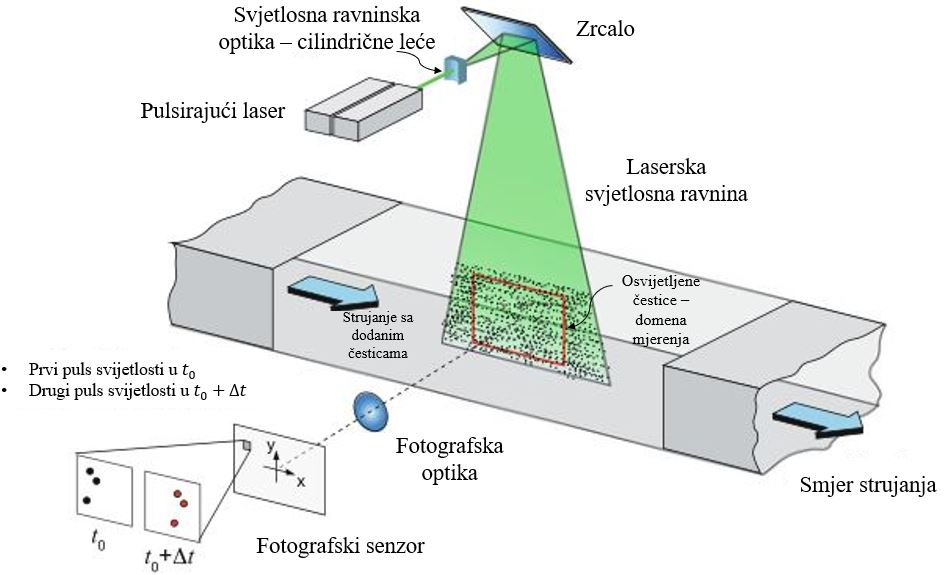
\includegraphics[width=14cm]{./2_DPIV/2_1PivSetup.jpg} 
	\caption{Eksperimentalni 2D PIV sustav \cite{raffel2018_book}}
	\label{sl:2.1}
\end{figure}
\par
U većini DPIV analiza snime se dvije fotografije (1 i 2) osvijetljene domene mjerenja u trenutcima $t_0$ i $t_0+\Delta t$. Brzine se stoga mogu dobiti uz pomoć parametara $\Delta t$ i udaljenosti koje su čestice prošle između dvije snimke 1 i 2 (pomak čestica). U DPIV pomak čestica proračunava se tako da se domena mjerenja podijeli u manja "prozore" mjerenja tzv. područja ispitivanja (\textit{eng. interrogation areas}). Svako područje ispitivanja sadrži svoju grupu čestica. Nakon podijele domene provodi se statistička analiza uz pomoć kros-korelacije (\textit{eng. cross-correlation}) svih podijeljenih prozora ispitivanja. Korelacija daje najvjerojatniji pomak grupe čestica koje se gibaju u ravnoj liniji između slika 1 i 2.
DPIV analiza ukratko se može podijeliti na 4 glavna koraka \cite{thielicke2014_article}: 
\begin{enumerate}[topsep=0pt, itemsep=0em]
	\item Akvizicija slika
	\item Pretprocesiranje slika (Softversko poboljšanje slika)
	\item Evaluacija slika
	\item Postprocesiranje PIV podataka
\end{enumerate}
\FloatBarrier
\section{Akvizicija slike}
Kako je PIV vizualna tehnika za analizu čestica, što znači da se PIV tehnikom brzina strujanja mjeri indirektno, prvi korak PIV procesa počinje fotografiranjem osvijetljene domene u koju su dodane čestice markeri. Da bi se omogućila što veća točnost PIV analize trebalo bi osigurati da dobivene slike budu što bolje kvalitete i da sadrže što manje šuma. U ovom radu prikazani su neki od najbitnijih parametara koji bi se trebali uzeti u obzir kod akvizicije slike. 
\subsection{Odabir čestica markera}
Fluidi su u većini slučajeva homogeni, pa je stoga brzine teško izmjeriti optičkim sredstvima. Zbog toga se uobičajeno u fluid dodaju razne reflektirajuće čestice. Obično odabir čestica kod tekućina ne predstavlja preveliki problem, međutim kod vizualizacije strujanja zraka, teško je pronaći čestice koje imaju sličnu gustoću kao i zrak. Prilikom odabira čestica treba uzeti u obzir sljedeće čimbenike i pretpostavke  \cite{raffel2018_book}:
\begin{description}[style=unboxed,leftmargin=0cm]
	\item[Distribucija čestica markera u struji fluida.] Poželjno je da distribucija čestica bude što homogenija.
	\item[Gustoća distribucije čestica markera unutar domene]. Na \textit{Slici \ref{sl:2.2}} mogu se primijetiti 3 različita tipa gustoće čestica, za koji bi se trebali primijeniti različite tehnike obrade.
	\begin{figure}[h]  
		\centering
		%\usepackage{graphicx}
		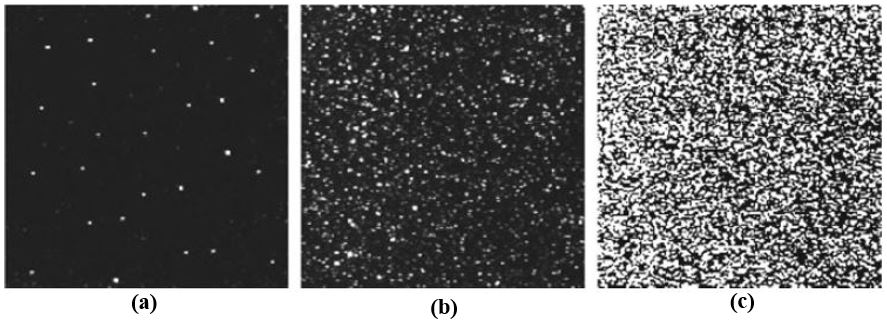
\includegraphics[width=14cm]{./2_DPIV/2_2GustocaDistribucijeCestica.jpg} 
		\caption{Tri moguća načina gustoće distribucije čestica \cite{raffel2018_book}:\\ \textbf{(a)} Niska gustoća (PTV)\\ \textbf{(b)} Srednja gustoća (PIV)\\ \textbf{(c)} Visoka gustoća čestica (LSV)}
		\label{sl:2.2}
	\end{figure}
	U slučaju niske gustoće (\textit{Slika \ref{sl:2.2}a}), moguća je detekcija i praćenje svake čestice zasebno. Radi toga niska gustoća distribucije za analizu zahtjeva neke od metoda praćenja objekata (markera). Stoga se ovaj način mjerenja naziva "\textit{mjerenje brzine praćenjem čestica}" (\textit{eng. PTV - Particle Tracking Velocimetry}). Za slučaj srednje gustoće distribucije čestica (\textit{Slika \ref{sl:2.2}b}) i dalje se može primijetiti svaka individualna čestica, međutim više nije moguće njihove praćenja zbog nesigurnosti da li je uistinu praćena čestica na sljedećoj slici ispravno i nedvosmisleno uočena. Ovakve fotografije analiziraju se uz pomoć statističkih PIV metoda (kros-korelacija). Kod slika sa visokom gustoćom distribucije čestica (\textit{Slika \ref{sl:2.2}c}) više nije moguće primijetiti svaku česticu posebno pošto dolazi do preklapanja i formiranja "mrlja" (\textit{eng. speckles}). U ovom slučaju mjerenje i analiza ovakvih fotografija naziva se "\textit{Laser Speckle Velocimetry}" (LSV).
	\item[Zaostajanje brzine (\textit{eng. velocity lag}).] Prilikom odabira čestica treba obratiti pažnju da li čestice vjerno prate gibanje svakog fluidnog elementa, barem do razine gdje se može zaključiti kako će rezultati mjerenja biti zadovoljavajući. Kod promatranja velikih domena strujanja, gdje se pojavljuju i veliki i mali gradijenti brzina, treba se pronaći kompromis između biranja većih i manjih čestica. Veće čestice će bolje raspršiti svjetlost, te će se vidjeti cijelo promatrano polje strujanja, ali ipak lokalno, mjesta gdje ima velikih promjena brzine će ostati neriješena. Glavni i najvažniji izvor grešaka kod korištenja čestica markera javlja se zbog djelovanja akceleracijskih sila (npr. gravitacija, centrifugalne sile) na česticu koja ima različitu gustoću od fluida, te će zbog toga ukratko biti objašnjen utjecaj ubrzanja \cite{raffel2018_book}. Kako postoji razlika u gustoćama između fluida $\rho$ i čestica tragača $\rho_\textup{č}$ prikazan je izraz za Stokes-ov zakon otpora \cite{Pehnec2020Predavanja} koji prikazuje zaostajanje brzine $\boldsymbol{U}_s$ između brzine čestice $\boldsymbol{U}_\textup{č}$ i brzine fluida $\boldsymbol{U}$. U izrazu se pretpostavlja da je čestica sfernog oblika, te struji u viskoznom fluidu pri jako malom Reynolds-ovom broju:
	\begin{equation}
		\boldsymbol{U}_{s}=\boldsymbol{U}_\textup{č}-\boldsymbol{U}=d_\textup{č}^2\dfrac{\rho_\textup{č}-\rho}{18\mu}\boldsymbol{a}
		\label{eqn:2.1}	
	\end{equation}
	gdje je $d_\textup{č}$ - promjer čestice, $\rho_\textup{č}$ - gustoća čestice, $\rho$ - gustoća fluida, $\mu$ - dinamička viskoznost fluida, $\boldsymbol{a}$ - ubrzanje.
	\par
	U slučaju naglog usporenja i velike razlike između gustoća fluida i čestica vremenski odziv $t$ brzine čestice $\boldsymbol{U}_\textup{č}$ ima trend eksponencijalnog raspada:
	\begin{equation}
		\boldsymbol{U}_\textup{č}(t)=\boldsymbol{U}\left[1-\exp\left(-\dfrac{t}{\tau_\textup{č}}\right)\right]
		\label{eqn:2.2}	
	\end{equation}
	gdje vrijeme odziva $\tau_\textup{č}$ glasi:
	\begin{equation}
		\tau_\textup{č}=d_\textup{č}^2\dfrac{\rho_\textup{č}}{12\mu}
		\label{eqn:2.3}
	\end{equation}
	Ako ubrzanje fluida nije konstantno ili Stokes-ov zakon otpora ne vrijedi (npr. za velike čestice ili veće brzine strujanja), rješenje jednadžbe \ref{eqn:2.3} više nije jednostavni eksponencijalni raspad. Razlog je u tome što jednadžbe strujanja (Navier-Stokes-ove jednadžbe) postaju nelinearne i sve su teže rješive. No unatoč tome $\tau_\textup{č}$ se i dalje može smatrati prikladnom mjerom za težnju čestice da uspostavi brzinsku ravnotežu sa fluidom. Na slici \ref{sl:2.3} prikazano je teoretsko vrijeme odziva (jednadžba \ref{eqn:2.2}) čestica različitih promjera kod "kvazi-trenutačnog" usporenja prilikom strujanja u zraku \cite{raffel2018_book}.
	\begin{figure}[h]  
		\centering
		%\usepackage{graphicx}
		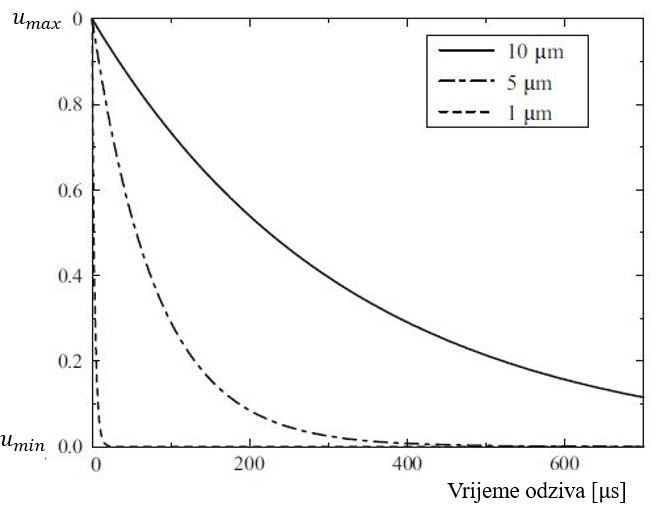
\includegraphics[width=9cm]{./2_DPIV/2_3VrijemeOdzivaCestica.jpg} 
		\caption{Teoretsko vrijeme odziva raspršenih uljnih čestica različitog promjera u zraku \cite{raffel2018_book}}
		\label{sl:2.3}
	\end{figure}
	\item[Utjecaj Brown-ovog gibanja.] U slučaju da su čestice markeri iznimno malog promjera (manje od 1 $\mu$m) može doći do tzv. Brown-ovog gibanja, gdje dolazi do efekta sudaranja, te miješanja čestica i fluida na mikro razinama (npr. gibanje čestica dima u zraku). Ovaj fenomen obično se pojavljuje pri $\mu$PIV mjerenjima, te dovodi do greški u kros-korelacijskoj analizi, zbog nesigurnosti u položaj čestica.
\end{description}
\FloatBarrier
\subsection{Osvjetljenje}
Kao osvjetljenje u PIV eksperimentima uobičajeno se primjenjuju pulsirajući laseri, zbog svoje sposobnosti da emitiraju monokromatsko svijetlo visokog energetskog intenziteta. Točkasti snop laserske svjetlosti jednostavno je transformirati u tanku ravninu (plahtu) koristeći jednu ili više cilindričnih leća \cite{raffel2018_book}, a osvjetljenje i snimanje korištenjem laserske ravnine onemogućuje kromatske aberacije. Danas je dostupno mnogo različitih lasera koji koriste razne tipove laserskih materijala, te različite načine energetskog upumpavanja. U PIV svrhe zbog svoje kompaktnosti i visoke efikasnosti najčešće se koriste "\textit{diodno upumpavani laseri čvrstom jezgrom}" (\textit{eng. DPSSL - diode pumped solid state lasers}).
\par
Najkorišteniji tip DPSSL lasera u PIV mjerenjima je Neodym-Yttrium-Aluminium-Garnet laser (Nd:YAG). Nd:YAG je laser s krutom jezgrom \cite{wiki:Nd:YAG} koji se sastoji od štapića itrij-aluminijevog granata (YAG), dopiranog atomima neodimija (Nd:\ch{Y3Al5O12)}. Radna valna duljina ovog lasera je 1064 nm (infracrveno zračenje), ali frekvencijskim dupliranjem, zraka koja napušta laser može se podesiti na valnu duljinu od 532 nm što odgovara zelenom spektru zračenja. Nd:YAG laseri mogu biti korišteni u pulsirajućem i kontinuiranom modu. Pulsirajući laseri ostvaraju veoma visoke snagu tijekom vrlo kratkih impulsa, što omogućuje smanjivanje efektivnog vremena ekspozicije kamere. Dok kontinuirani laseri zahtijevaju dulja vremena ekspozicije kako bi ostvarili zadovoljavajuću količinu svjetla, a dulja ekspozicija dovodi do pretjeranog zamućenja gibanja čestice. Zamućene čestice nisu poželjne zbog kvalitete kros-korelacijske obrade (poželjno je da svaka slika doslovno zamrzne gibanje čestica). Ipak prednost kontinuiranih lasera je u tome da ne zahtijevaju dodatni hardware za sinkronizaciju sa brzim kamerama, za razliku od pulsirajućih lasera, gdje je sinkronizacija kamere i lasera neizbježna.
\subsection{Snimanje}
Osvijetljena ravnina u PIV analizi snimana je kamerom kojoj optička os "udara" okomito na osvijetljenu ravninu. Za PIV snimke generalno su potrebne jako kvalitetne leće zbog toga što leveli svjetlosti znaju biti relativno niski, te su potrebni veliki otvori blende da uhvate što više svjetla. Znatan napredak PIV analize omogućen je pojavom digitalnih kamera sa CCD ili CMOS foto čipovima. Ove kamere omogućile su instant analizu strujanja i povratnu informaciju o kvaliteti slike. Elektronske kamere dostupne su cijelom području rezolucija, osjetljivosti, brzine zatvarača (\textit{eng. shutter speed}), brzine snimanja (\textit{eng. frame rate}), itd.. Prilikom odabira kamere za određena PIV mjerenja treba uzeti u obzir sljedeće eksperimentalne karakteristike: područje brzina strujanja koje se promatraju, ponovljivost eksperimenta, te intenzitet osvjetljenja. U \textit{Tablici \ref{tab:2.1}} prikazan je općeniti sažetak najčešćih eksperimentalnih situacija, te tipa kamere koji se preporučuje koristiti.
\begin{table}[h]
	\centering
	\caption{Preporuka pri odabiru kamere za PIV mjerenja ovisno o brzini strujanja, ponovljivosti eksperimenta i jačini osvjetljenja \cite{stamhuis2006basics}}
	\begin{tabular}{|c|c|c|c|}
		\hline
		\rowcolor[HTML]{9B9B9B} 
		\begin{tabular}[c]{@{}c@{}}\textbf{Brzina} \\ \textbf{strujanja}\end{tabular} & \begin{tabular}[c]{@{}c@{}}\textbf{Intenzitet} \\ \textbf{osvijetljenja}\end{tabular} & \textbf{Ponovljivost} & \textbf{Tip kamere}                                                                                                                  \\ \hline
		&                                                                     & Dobra        & \begin{tabular}[c]{@{}c@{}}Kamera sa dvostrukom \\ (višestrukom) ekspozicijom\end{tabular}                                  \\ \cline{3-4} 
		\multirow{-2}{*}{Brzo}                                      & \multirow{-2}{*}{Visok}                                             & Loša         & Brza kamera                                                                                                                 \\ \hline
		&                                                                     & Dobra        &                                                                                                                             \\ \cline{3-3}
		\multirow{-2}{*}{Sporo}                                     & \multirow{-2}{*}{Nizak}                                             & Loša         & \multirow{-2}{*}{\begin{tabular}[c]{@{}c@{}}Progressive scan kamera \\ (normalna ili srednja brzina snimanja)\end{tabular}} \\ \hline
	\end{tabular}
\label{tab:2.1}
\end{table}
\par
Progresivne scan kamera omogućuje snimanje slika brzinom od 25-30 fps pa sve do 100 fps (\textit{frames per second}). Ove vrste kamera se zbog dugačkog perioda između kadrova koriste pri niskim PIV brzinama. Brze kamere imaju mogućnost snimanja do 1000 fps, te su ove kamere izvrsne za brza strujanja gdje nema ponovljivosti (npr. snimanje strujanja oko ptica). Korištenje brze kamere u PIV analize (za neke slučajeve) je poznato i kao vremenski razriješeni PIV (\textit{eng. time-resolved PIV}). Kamera sa dvostrukom ekspozicijom ima mogućnost snimanja dvije ekspozicije (kadra) unutar iznimno kratkog perioda. Nakon snimanja obje ekspozicije se prebace na računalo, te je kamera spremna za snimanje novog para dvije ekspozicije. Period između para dvije ekspozicije može biti ispod 500 ns, no zato period između parova ekspozicija je dosta duži (0.1 do 0.5 s), ovisno o sustavu transfera slika na računalo (ili unutarnju memoriju). Zbog toga više-ekspozicionirane snimke su prikladne za PIV u kojem su brzine strujanja visoke ali i postoje ponovljivi uzorci strujanja.
\FloatBarrier
\section{Pretprocesiranje slike}
U DPIV analizi treba omogućiti što kvalitetniju procjenu brzine kako bi se osigurala najveća moguća kvaliteta mjerenja \cite{thielicke2014_article}. Jedan od uobičajenih pristupa je digitalno poboljšanje slike prije nego se dogodi sami postupak korelacije. Varijacije intenziteta slike snažno utječu na signal korelacije. Mjesta gdje su čestice bolje osvijetljene imaju puno veći utjecaj u korelaciji od mjesta gdje su čestice manje osvijetljene. Također nejednoliko osvijetljenje (zbog ne-uniformne distribucije laserske svjetlosti, varijacija između laserskih impulsa, nepravilno oblikovanih čestica, kretanja izvan ravnine,...) unose šum u korelacijsku ravninu. Iz tog razloga ulazne slike se gotovo uvijek poboljšavaju prije same evaluacije. Glavni cilj poboljšanja slike je primjena raznih tehnika kako bi se dovelo do većeg kontrasta u slici, te do toga da intenzitet čestica u slici dovede do slične razine signala tako da sve čestice imaju sličan doprinos u korelacijskoj funkciji. U idealnim uvjetima PIV slike bi se trebale sastojati od svijetlih čestica promjera 2-3 pixela koje se nalaze na crnoj površini. Na taj način korelacijska efikasnost bi se mogla dovesti na sub-pixelsku točnost \cite{mendez2017pod}. U ovom potpoglavlju biti će objašnjeni neke od pretprocesorskih tehnika koje se koriste u ovom radu i implementirane su u PIVlab softver.
\par
Jedan od načina postizanja bolje kvalitete slike je stacionarno "\textit{oduzimanje pozadine}" (\textit{eng. background subtraction}). Ova tehnika  smanjuje učinke laserskog odbljeska i ostalih stacionarnih značajki slike. Može se izvesti tako da se pozadinska slika snimi prije samog dodavanja čestica markera, ili ako to nije moguće, izračunavanjem slike prosječnog ili  minimalnog intenziteta iz dovoljno velik broja PIV snimki (najmanje 20-50). \cite{raffel2018_book}.
\par
Drugi način poboljšanja slike je zasnovan na "\textit{visoko-propusnom filtriranju}" (\textit{eng. high-pass filtering}) poznatom kao i izoštravanje fotografije. Ovom tehnikom pozadinske varijacije sa malom prostornom frekvencijom se uklanjaju ostavljajući tako slike čestica nepromijenjene. U praksi ovo se radi na način da se izračuna nisko-propusna verzija originalne slike i oduzme se od svoje originalne slike. Bitno je da širina primijenjenog filtra (\textit{eng. filter kernel}) bude veća od promjera čestica ($k_{\textup{filtra}}>d_\textup{č}$).
\par
Zajedno sa visoko-propusnim filtriranjem često se koristi i \textit{binarizacija slike} (\textit{eng. image binarization}) poznato kao i "\textit{thresholding}". Kao rezultat se dobije slika (obično crno-bijela) gdje sve čestice imaju jednak intenzitet i samim time jedak doprinos korelacijskoj funkciji. Međutim ova tehnika dovodi do povećavanja nesigurnosti u mjerenju, pa bi se trebala koristiti s oprezom.
\par
Korištenje filtra niske širine, "\textit{nisko-propusnog filtra}" (\textit{eng. low-pass filter}) može biti prikladno za uklanjanje visoko frekvencijskog šuma (npr. šum fotoaparata, pixel anomalije,...).
\subsection{Prilagodljivo rastezanje kontrasta}
\textit{Prilagodljivo rastezanje kontrasta} \cite{wiki:Adaptive_histogram_equalization} ili \textit{prilagodljivo izjednačavanje histograma} (\textit{eng. AHE - adaptive histogram equalization}) je tehnika obrade slike kojom se poveća kontrast slike. Razlikuje se od običnog rastezanja kontrasta (\textit{Slika \ref{sl:2.4}}) u kojem se globalno poveća kontrast, pa dolazi do toga da je u nekim područjima slike, kontrast optimalno definiran, a u drugim područjima nastaje mnogo šuma. AHE radi na način da se računa više histograma koji odgovaraju određenom lokalnom području slike. Na taj način kontrast slike optimalno se poboljša za svako područje slike, međutim i dalje može doći do pretjeranog pojačanja šuma u relativno homogenim područjima slike. Kako bi se to spriječilo u PIVlab softveru koristi se varijanta AHE-a koja se naziva \textit{kontrast ograničeno prilagodljivo izjednačavanje histograma} (\textit{eng. CLAHE - contrast limited adaptive histogram equalization}). CLAHE algoritam je predstavljen 1987 kao algoritam koji bi povećao "čitljivost" medicinskih fotografija.
\begin{figure}[h]  
	\centering
	%\usepackage{graphicx}
	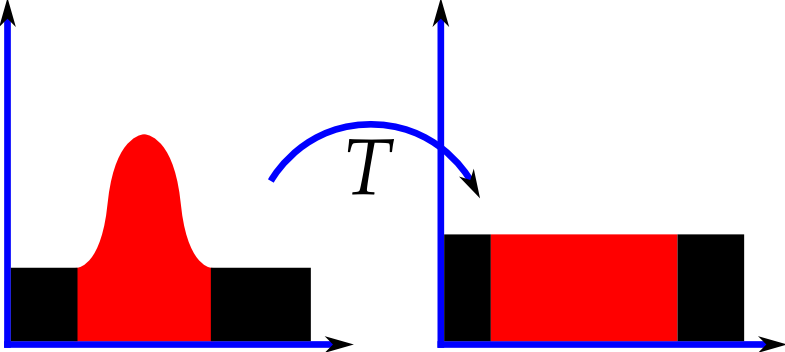
\includegraphics[width=8cm]{./2_DPIV/2_4Histogram.jpg} 
	\caption{Primjer histograma prije i nakon izjednačavanja \cite{wiki:Histogram_equalization}}
	\label{sl:2.4}
\end{figure}
\par
Prednost CLAHE algoritma u odnosu na AHE je da limitira pojačanje kontrasta u područjima koja nemaju nagle promjene. Ovo je jako bitno kod DPIV analize zbog toga što uniformna ekspozicija cijele slike često ne može biti osigurana \cite{adrian2011_book}, prvenstveno radi toga što laserska ravninska zraka ima normalnu (Gauss-ovu) distribuciju. U CLAHE-e algoritmu, kontrast svakog područja je optimiziran izjednačavanjem histograma tako da rezultirajuća distribucija odgovara histogramu ravnog oblika (\textit{eng. flat shaped histogram}) u rasponu od 0 do 255 za 8-bitne slike. Na taj način područja sa niskom ekspozicijom i područja sa visokom ekspozicijom su neovisno optimizirana. Nakon izjednačavanja histograma sva susjedna područja izjednačena su uz pomoć bilinearne interpolacije, što daje sliku koja nema nikakvih vidljivih granica između lokalnih područja. CLAHE algoritam osjetno poboljšava vjerojatnost detekcije vektora brzina u eksperimentalnim slikama za $4.7 \pm 3.2\%$ \cite{thielicke2014_phd}. Primjer rezultata primjene CLAHE i ostalih pretprocesorskih tehnika prikazan je na \textit{Slici \ref{sl:2.5}}.
\FloatBarrier
\subsection{Visoko-propusno filtriranje}
Nehomogeno osvjetljenje (npr. uzrokovano refleksijama od razne objekte ili čestice prilikom akvizicije slike), jako utječe na korelacijsku funkciju. Kao što je već ranije spomenuto, ova vrsta nisko-frekvencijske pozadinske informacije može biti uklonjena primjenom visoko-propusnog filtra - izoštravanje slike (\textit{eng. HPF - high-pass filter}) koji sačuva visoko-frekvencijske informacije osvijetljenih čestica. HPF se računa primjenom nisko-propusnog filtra na sliku (zamućenje slike), te oduzimanjem rezultata do originalne slike. HPF naglašava informacije o česticama na slici, te potiskuje svaku informaciju o niskoj frekvenciji. HPF filtri poznati kao "\textit{kerneli}" obično su matrice veličine od $7 \times 7$ do $15 \time 15$ (\textit{eng. kernel filter}) koje se konvoluiraju sa originalnom slikom. Kernel visoko-propusnog filtra je dizajniran tako da poveća intenzitet središnjeg pixela, relativno u odnosu na susjedne pixele.
\begin{figure}[h]  
	\centering
	%\usepackage{graphicx}
	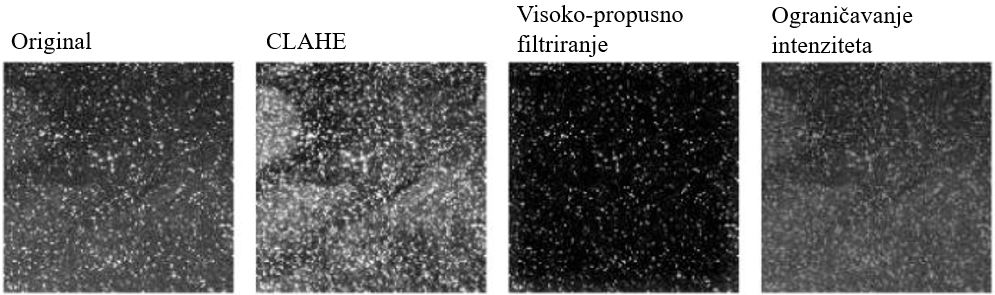
\includegraphics[width=16.5cm]{./2_DPIV/2_5IzostravnjeSlike.jpg} 
	\caption{Primjer dobivenog efekta nakon primjene u tekstu opisanih pretprocesorskih tehnika \cite{thielicke2014_article}}
	\label{sl:2.5}
\end{figure}
\FloatBarrier
\subsection{Ograničavanje intenziteta}
Čest izvor grešaka u DPIV analizi je prisutnost jako svijetlih mrlji unutar PIV slika \cite{shavit2007intensity}. Svijetle mrlje su okarakterizirane intenzitetom sivih tonova mnogo većim od srednje vrijednosti intenziteta slike. Pomak svijetlih mrlja u odnosu na ostale čestice više pridonosi korelacijskom signalu unutar područja ispitivanja, što dovodi do veće pristranosti u konačnom vektoru brzina. \textit{Ograničavanje intenziteta} (\textit{eng. Intensity Capping}) je tehnika poboljšanja slike koja daje bolje PIV rezultate u slučaju da se na slici nalaze svijetle mrlje. Tehnikom ograničavanja intenziteta korisniku je omogućeno određivanje gornje granice intenziteta sivih tonova u području ispitivanja. Svi pixeli koji premaše zadani prag zamijene se iznosom gornje granice. Računanje pomaka u tom slučaju bolje predstavlja pomak svih čestica u području ispitivanja, a pristranost prema svijetlim mrljama je minimizirana. Ograničavanje intenziteta poboljšava detekciju ispravnih vektora brzina za $5.2 \pm 2.5\%$. Na \textit{Slici \ref{sl:2.6}a} prikazana je originalna PIV fotografija sa svojim rezultirajućim poljem brzina (dolje), te PIV slika nakon primjene ograničavanja intenziteta (\textit{Slika \ref{sl:2.6}b}) sa poljem brzina, također. Sa slika je vidljivo kako primjena ograničavanja intenziteta je mnogo utjecala na pojavu individualnih pristranih vektora brzina (Napomena - na slikama su prikazani samo dijelovi cijele domene radi estetskih razloga, pa zbog toga same slike i rezultati nisu u mjerilu).
\begin{figure}[h]  
	\centering
	%\usepackage{graphicx}
	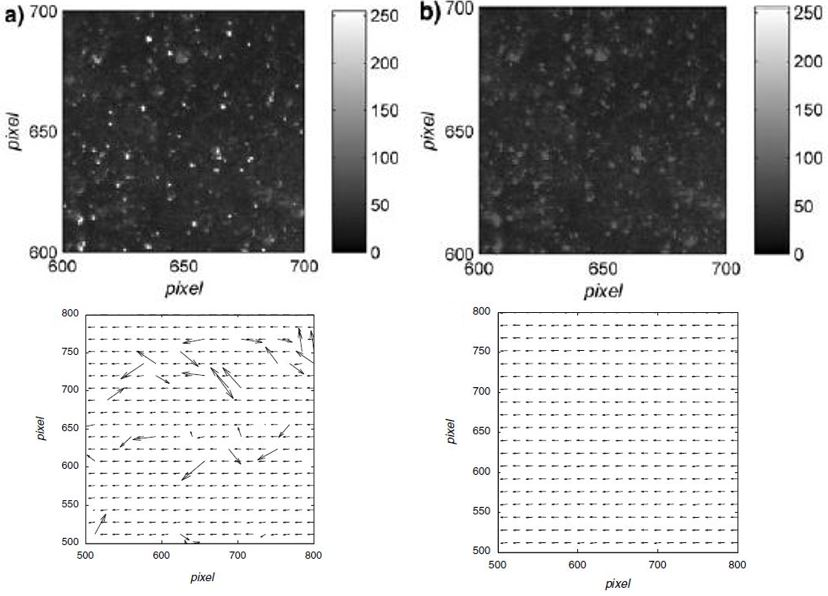
\includegraphics[width=11cm]{./2_DPIV/2_6IntensityCapping.jpg} 
	\caption{Primjer primjene tehnike ograničavanja intenziteta, te dobivena polja brzina nakon analize kros-korelacijom \cite{shavit2007intensity}}
	\label{sl:2.6}
\end{figure}
\FloatBarrier
\section{Evaluacija slike}
Najosjetljiviji i najvažniji dio efikasnosti i točnosti DPIV analize je sama kros-korelacija PIV fotografija. Korelacija je bilo koji statistički odnos, te predstavlja međusobnu povezanost između različitih pojava predstavljenih vrijednostima dviju varijabli. Pri tome povezanost znači da je vrijednost jedne varijable moguće sa određenom vjerojatnošću predvidjeti na osnovi saznanja o vrijednosti druge varijable \cite{wiki:Correlation}. U 1D obradi signala kros-korelacija je mjera sličnosti dviju serija kao funkcija relativnog pomaka jedne serije u odnosu na drugu seriju, što je poznato kao i "\textit{klizajući skalarni produkt}" (\textit{eng. sliding dot product} ili \textit{sliding inner-product}). Glavni cilj kros-korelacije u DPIV analizi je evaluacija PIV fotografija kako bi se odredio pomak između dva lokalna uzorka nasumično distribuiranih čestica, koje su spremljene kao 2D distribucija sivih tonova. Teoriju 1D kros korelacije iz obrade signala lako je proširiti na 2D (npr. ravninska distribucija sivih tonova) ili 3D (prostorna distribucija) \cite{raffel2018_book}.
\par
Kao što je već spomenuto ranije prvi korak DPIV evaluacije je podijeliti PIV snimke na manja područja (prozore) ispitivanja (\textit{eng. interrogation areas (windows)}). Prozor ispitivanja predstavlja lokalni uzorak čestica PIV fotografije koji je opisan jednim vektorom brzine, pa prema tome veličina prozora ispitivanja određuje do koje razine rezolucije je dobiveno polje brzina.
\par
Neka se sada pretpostavi kako su snimljene dvije uzastopne PIV snimke iz stroboskopom osvijetljene svjetlosne ravnine (za početak neka budu zanemareni efekti kašnjenja čestica, 3D gibanja,...). Iz dvije uzastopne snimke sve što je moguće izmjeriti je pravocrtni pomak u vremenu (za dobivanje informacija o ubrzanju i zakrivljenosti strujanja, potrebno je više snimki). Ove dvije snimke (\textit{Slika \ref{sl:2.7}}) mogu dati vektor pravocrtnog pomaka, gdje je svaki vektor formiran iz analize gibanja lokalnog uzorka čestica iz prozora ispitivanja.
\begin{figure}[h]  
	\centering
	%\usepackage{graphicx}
	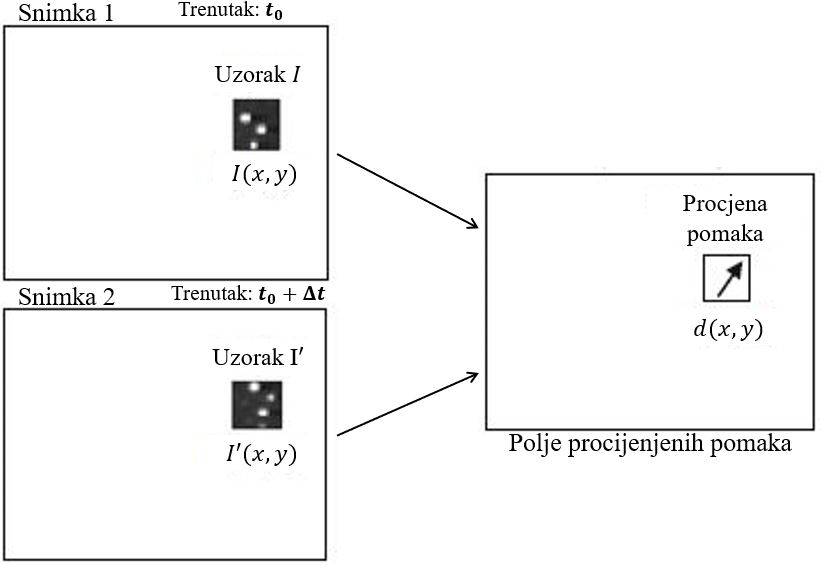
\includegraphics[width=11cm]{./2_DPIV/2_7OpisGibanja.jpg} 
	\caption{Konceptualni prikaz povezivanja kadrova snimki 1 i 2 i dobivanja vektora pomaka\cite{raffel2018_book}}
	\label{sl:2.7}
\end{figure}
\par
U suštini kros-korelacija je tehnika statističkog povezivanja uzorka iz snimke 1 (snimljene u trenutku $t_0$) sa uzorkom iz snimke 2 (snimljene u trenutku $t_0 + \Delta{t}$). Ova statistička tehnika implementirana je uz pomoć funkcije diskretne kros-korelacije \cite{raffel2018_book}:
\begin{equation}
	R_{II}(x, y) = \sum_{i=-M}^{M}\sum_{j=-N}^{N}I(i, j)I'(i+x, j+y)
	\label{eqn:2.4}
\end{equation}
gdje su varijable $I$ i $I'$ odgovarajući prozori ispitivanja (vrijednosti intenziteta) iz slika (ekspozicija) 1 i 2. Za dani pomak diskretna kros-korelacija stoga mjeri "poklapanje" prozora ispitivanja $I$ sa prozorom $I'$. Lokacija najvećeg vrha intenziteta (najveća vrijednost) u rezultirajućoj korelacijskoj matrici $R_{II}$ daje najvjerojatniji mogući pomak čestica iz snimke 1 u snimku 2.
\par
Jednadžba \ref{eqn:2.4} rješava se na dva načina. Najizravniji pristup je da se korelacijska matrica izračuna u prostornoj domeni, ovaj pristup naziva se direktna kros-korelacija (ili konvolucijsko filtriranje). Drugi pristup dobivanja korelacijske matrice je računanje u frekvencijskoj domeni (diskretna Fourier-ova transformacija - DFT). DFT se računa koristeći FFT algoritam (\textit{eng. Fast Fourier Transform}) i u principu je brži način dobivanja korelacijske matrice, za razliku od direktnog računanja koje je sigurnije i točnije.
\FloatBarrier
\subsection{Direktna prostorna kros-korelacija}
Direktna kros-korelacija (DKK) računa korelacijsku matricu u prostornoj domeni. U DKK , prozori ispitivanja $I$ i $I'$ obično su različitih veličina. Ako se odabere da je područje $I'$ bude duplo veće od područja $I$, pomicanje čestica do polovine veličine $I$ neće rezultirati gubitkom podataka i pružit će pouzdanu matricu korelacije sa niskim pozadinskim šumom (\textit{Slika \ref{sl:2.8}}).
\begin{figure}[h]  
	\centering
	%\usepackage{graphicx}
	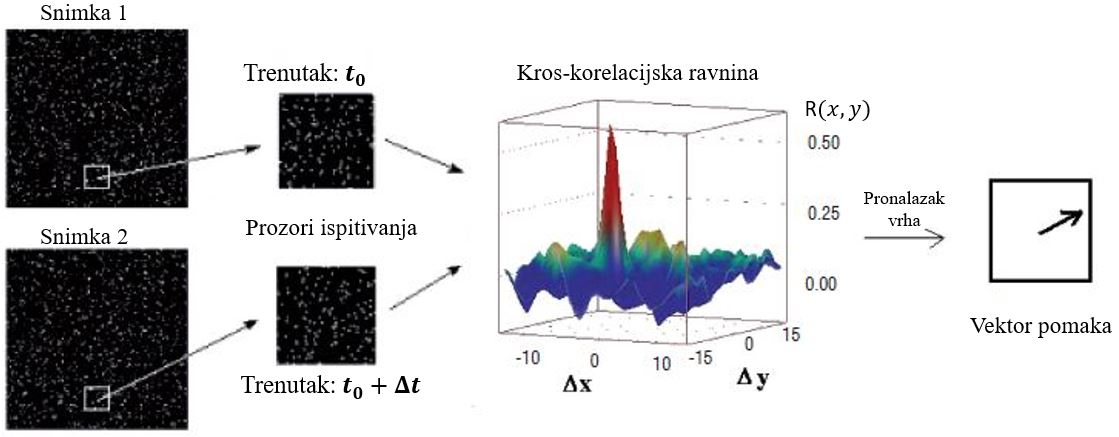
\includegraphics[width=14cm]{./2_DPIV/2_8KrosKorelacijskaRavnina.jpg} 
	\caption{Konceptualni prikaz povezivanja kadrova snimki 1 i 2 i dobivanja vektora pomaka\cite{brossard2009_article}}
	\label{sl:2.8}
\end{figure}
\par
Direktna kros-korelacija prozor ispitivanja $I$ iz jednadžbe \ref{eqn:2.4} linearno "pomiče" oko prozora $I'$ bez da prijeđe preko ruba $I'$. Za svaki odabir pomaka uzorka $(x, y)$, dobije se vrijednost intenziteta kros-korelacije $R_{II}(x, y)$, što je u suštini suma umnožaka intenziteta svih pixela koji se preklapaju. Ako se ova operacija izvede na rasponu pomaka ($-M \leq x \leq M$; $-N \leq y \leq N$), dobije se kros-korelacijska ravnina veličine $(2M+1) \times (2N+1)$. Ovaj postupak pomicanja grafički je prikazan na \textit{Slici \ref{sl:2.9}}, gdje je dan primjer sa $4 \times 4$ prozorom $I$ koji je koreliran sa $8 \times 8$ prozorom $I'$ koji skupa formiraju $9 \times 9$ korelacijsku matricu $R$. 
\begin{figure}[h]  
	\centering
	%\usepackage{graphicx}
	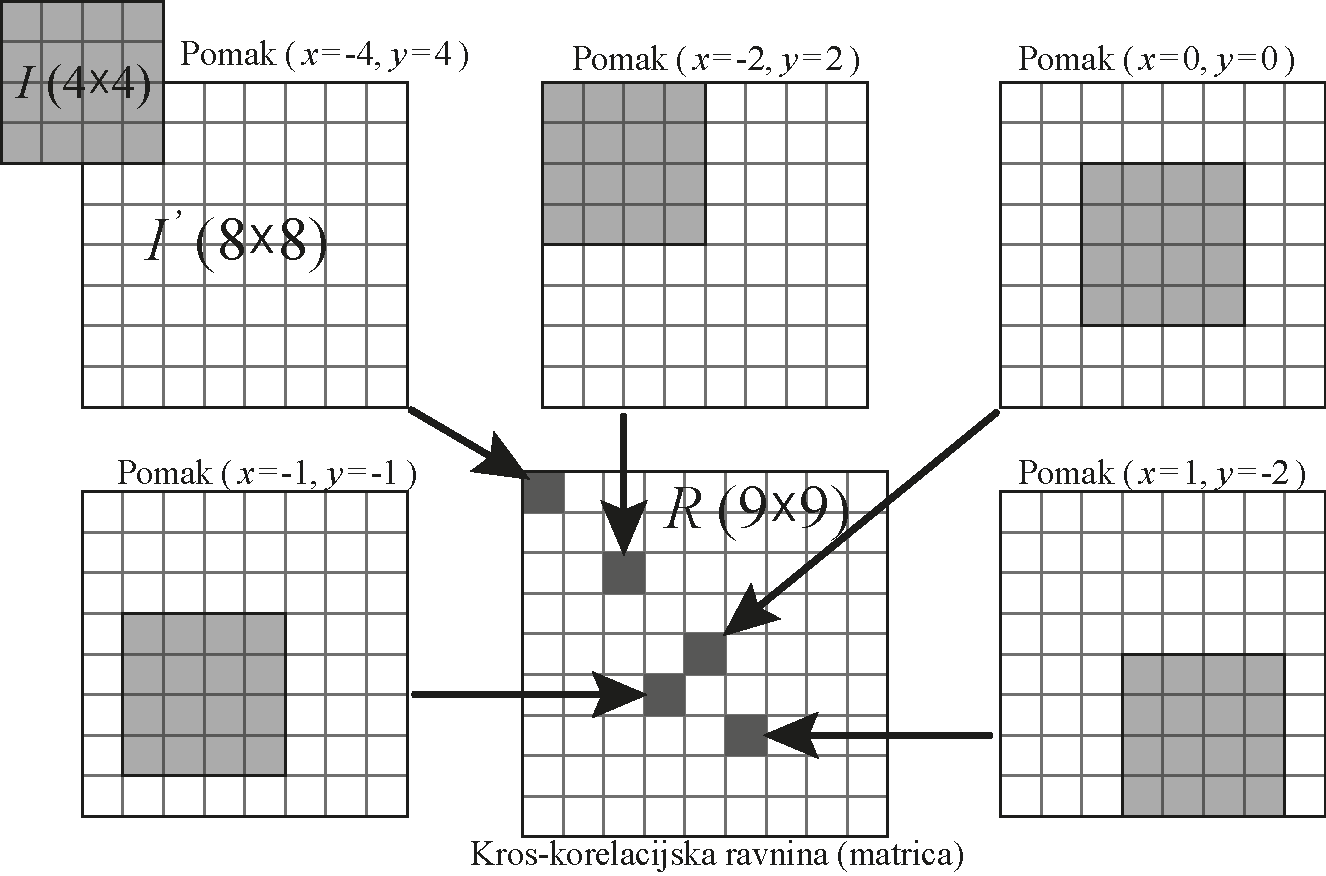
\includegraphics[width=16cm]{./2_DPIV/2_9PostupakPomicanja.pdf} 
	\caption{Primjer formacije korelacijske ravnine koristeći DKK}
	\label{sl:2.9}
\end{figure}
\par
Za vrijednosti pomaka gdje se prozor ispitivanja $I$ poklopi sa prozorom $I'$ suma umnožaka intenziteta pixela imat će najveću vrijednost, te će ta vrijednost signalizirati pomak čestica. Ukratko, kros-korelacijska funkcija (jednadžba \ref{eqn:2.4}) statistički mjeri stupanj preklapanja između dva prozora ispitivanja za dani pomak. U današnjim PIV evaluacijama tipične veličine prozora ispitivanja su $32 \times 32$ pixela (ili $16 \times 16$ pixela).
\par
Iz implementacije DKK mogu se uočiti dva nedostatka \cite{raffel2018_book}. 
\begin{itemize}[topsep=0pt, itemsep=0em]
	\item Prvo, broj računanja po korelaciji eksponencijalno (kvadratno) raste  sa povećanjem prozora ispitivanja. Tipična PIV analiza koristi nekoliko tisuća pixela, dok je raspon ispitivanja oko $\pm 20$ pixela, što znači da se mora izvršiti preko milijun multiplikacija i zbrajanja kako bi se formirala samo jedna korelacijska matrica. Ako se uzme u obzira da se mora izračunati nekoliko tisuća vektora pomaka računalna snaga počinje igrati veliku ulogu u računanju korelacijske matrice. Jedan od načina zaobilaska problema kvadratnog rasta računanja je korištenje Fourier-ove transformacije i računanja u frekvencijskoj domeni, što je i objašnjeno u daljnjem radu. No ipak u zadnje vrijeme dolazi do razvoja računalne tehnologije i tehnike paralelnog računanja na grafičkim jedinicama (GPU) što značajno pridonose brzini kalkulacija, te potencijalno čini DKK dovoljno brzim za primjenu.
	\item Drugo, kros-korelacijskom metodom dobiju se samo pravocrtni pomaci - \textit{metoda prvog stupnja} (\textit{eng. first order method}), što znači da je ne moguće izvući informacije o rotacijama i deformacijama. Ovo znači da se veličina prozora ispitivanja mora odabrati dovoljno malenom da se može smatrati kako su efekti višeg stupnja (rotacija, deformacija) zanemarivi.
\end{itemize}
\FloatBarrier
\subsection{Računanje korelacijske funkcije u frekvencijskoj domeni}
Glavni problem direktnom računanju korelacijske matrice (potrebna računalna snaga) može se riješiti tako da se korelacijska matrica izračuna u frekvencijskoj domeni koristeći diskretnu Fourier-ovu transformaciju (DFT). Na taj način bi se iskoristila prednost  korelacijskog teorema koji tvrdi da kros-korelacija dviju funkcija je ekvivalentna kompleksno-konjugiranom umnošku njihove Fourier-ove transformacije:
\begin{equation}
	R_{II} \iff \hat{I}\cdot \hat{I}'^*
	\label{eqn:2.5}
\end{equation}
gdje su $\hat{I}$ i $\hat{I}'$ Fourier-ove transformacije funkcija $I$ i $I'$. U praksi
Fourier-ova transformacija za diskretne podatke se efikasno računa koristeći FFT (\textit{eng. fast Fourier transform}) algoritam koji smanjuje računanje sa $O[N^2]$ operacija na $O[N\log N]$ operacija. Tako se zahtjevni 2-dimenzionalni korelacijski proces može svesti na računanje 2D FFT-ova jednako velikih uzoraka ispitivanja sa snimke nakon čega slijedi kompleksno-konjugirano množenje rezultirajućih Fourier-ovih koeficijenata. Dobiveni koeficijenti se onda inverznom Fourier-ovom transformacijom vrate u prostornu domenu (kros-korelacijsku ravninu) koja ima istu prostornu dimenziju kao i ulazne slike 1 i 2 (\textit{Slika \ref{sl:2.10}}).
\begin{figure}[h]  
	\centering
	%\usepackage{graphicx}
	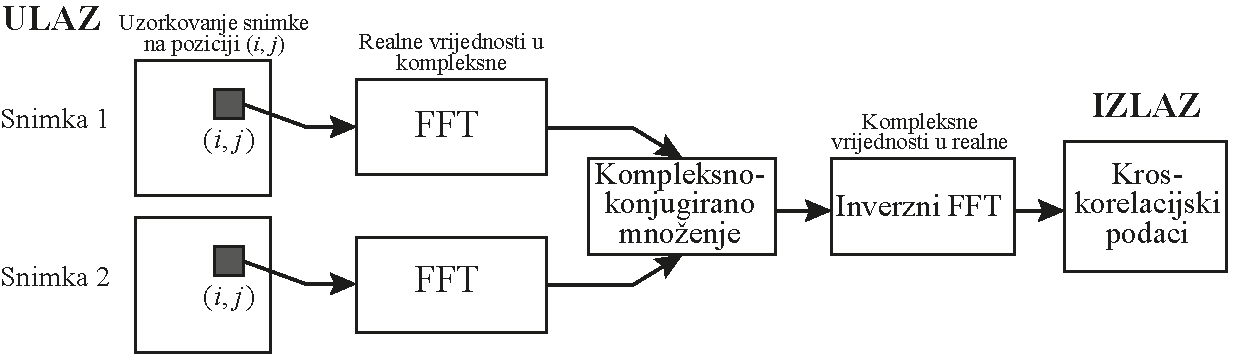
\includegraphics[width=16.5cm]{./2_DPIV/2_10FFT_postupak.pdf} 
	\caption{Računanje kros-korelacije koristeći FFT \cite{raffel2018_book}}
	\label{sl:2.10}
\end{figure}
\par
DFT pristup koristi prozore ispitivanja iz snimki 1 i 2 koji su iste veličine što rezultira određenim gubitkom informacija, koji se registrira pojavom pozadinskog šuma u korelacijskoj matrici \cite{thielicke2014_article}. Pozadinski šum u korelacijskoj ravnini komplicira detekciju vrhova, što smanjuje točnost mjerenja. Dodatni problem korištenja DFT je to što FFT po definiciji pretpostavlja da su ulazni podaci (prozori ispitivanja) periodični, to jest da se ponavljaju u svim smjerovima. Ako je pomak čestica veći od polovice veličine prozora ispitivanja, vrh u korelacijskoj ravnini je "presavijen" u matrici, te se pojavi na suprotnoj strani korelacijske ravnine. Za točni pomak $d_{x,to\textup{č}no}>N/2$, izmjereni pomak će iznositi $d_{x,izmjereno}=d_{x,to\textup{č}no}-N$. U tom slučaju kriterij uzorkovanja (Nyquist-Shanon-ov teorem) neće biti ispunjen što dovodi do pod-uzorkovanja podataka (\textit{eng. aliasing}). Stoga, pomak čestica obavezno mora biti manji od polovice veličine prozora ispitivanja. Preporuka je da pomak bude jedna četvrtina veličine prozora ispitivanja (\textit{eng. one-quarter rule}), kako bi se pozadinski šum u korelacijskoj matrici održao na niskim razinama. Još jedan način na koji se pozadinski šum može minimizirati, uz povećanje prozora ispitivanja je da se smanji vrijeme između snimki kamere. Također moguće je da se provode više prolaza diskretne Fourier-ove transformacije (DFT) na isti set podataka (prozora ispitivanja), što značajno povećava omjer signal-šuma \cite{thielicke2014_article}. Nakon prve DFT analize (prvog prolaza), dobivena cjelobrojna vrijednost se koristi kao podatak koji će promijeniti veličinu prozora ispitivanja u sljedećem prolazu, te tako minimizirati gubitak informacija zbog pomaka čestica. Nadalje, kako bi se dodatno poboljšao DFT  algoritam moguće je poboljšati mrežu ispitivanja sa svakim prolazom. Prvi prolaz bi koristio veće prozore ispitivanja te bi tako pronašao i veće pomake čestica. U sljedećim prozorima, prozori ispitivanja bi se smanjili i pomakli u isto vrijeme što bi dovelo do veće prostorne rezolucije, te većeg raspona mjerenih brzina.
\par
Još jedna negativna strana periodičnosti korelacijskih podataka je u tome da korelacijske procjene budu pristrane. Sa sve većim pomacima, sve se manje podataka međusobno korelira budući da periodički kontinuirani podaci korelacijskog uzorka ne daju nikakav doprinos korelacijskoj vrijednosti. Vrijednosti na rubu korelacijske ravnine računaju se samo iz preklapajuće polovice podataka i treba ih ispravno ponderirati. Ukoliko podaci nisu ispravno ponderirani, procjena pomaka biti će pristranija nižoj vrijednosti (\textit{Slika \ref{sl:2.11}}). Snimke sa većim česticama daju šire korelacijske vrhove, te samim time i veće greške pristranosti. U poglavlju koje opisuje detekciju korelacijskih vrhova ukratko je opisana pogodna funkcija kojom je moguće rješavanje problema pristrane pogreške
\begin{figure}[h]  
	\centering
	%\usepackage{graphicx}
	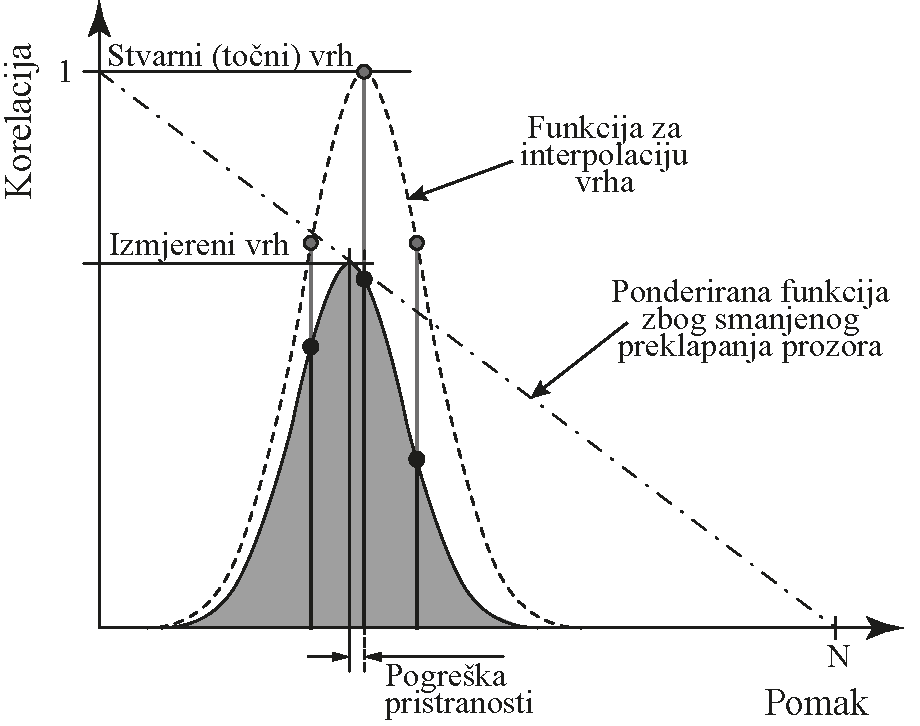
\includegraphics[width=10cm]{./2_DPIV/2_11BiasError.pdf} 
	\caption{Pogreška pristranosti u računanju kros-korelacije koristeći FFT \cite{raffel2018_book}}
	\label{sl:2.11}
\end{figure}
\par
Do sada je pretpostavljeno kako čestice unutar prozora ispitivanja imaju uniformno gibanje. U stvarnom strujanju čestice su podvrgnute raznim smicanjima i rotacijama, što dovodi do ne-uniformnog gibanja koje proširuje intenzitete vrhova u korelacijskoj ravnini, te rezultira lošijim rezultatima. Postoji nekoliko tehnika koje uzimaju u obzir transformaciju prozora ispitivanja (višestruki prolaz, poboljšanje mreže prozora, \textit{tehnika deformacije prozora}). U PIVlab softveru se primjenjuje sljedeći postupak: Analiza započinje sa standardnim DFT algoritmom. Prvi prolaz DFT-a daje informacije o pomaku centra svakog prozora ispitivanja. Kada dođe do preklapanja područja jedno preko drugo za npr. 50\% dobije se dodatna informacija o pomaku na granicama i uglovima svih područja ispitivanja (sveukupno devet pozicija, \textit{Slika \ref{Tehnika deformacije prozora} lijevo}). Uz pomoć dobivene informacije izračuna se pomak svakog pixela unutar prozora ispitivanja koristeći bilinearnu interpolaciju. Nakon toga, područje ispitivanja B se deformira prema dobivenom pomaku (\textit{Slika \ref{Tehnika deformacije prozora} desno}) koristeći bilinearnu interpolaciju ili spline interpolaciju (preciznije, ali sporije). Sljedeći prolaz ispitivanja korelira originalno područje A sa deformiranim područjem B. Akumuliraju se preostale informacije o pomaku prilikom svakog prolaza. Nakon nekoliko prolaza, deformirano područje ispitivanja B izgleda gotovo identično kao originalno područje A, te je pomak određen sa velikom preciznošću. Između prolaza, ali ne nakon posljednjeg prolaza, informacije o brzini su izglađene i potvrđene, a informacije koje nedostaju su interpolirane.
\begin{figure}[h]  
	\centering
	%\usepackage{graphicx}
	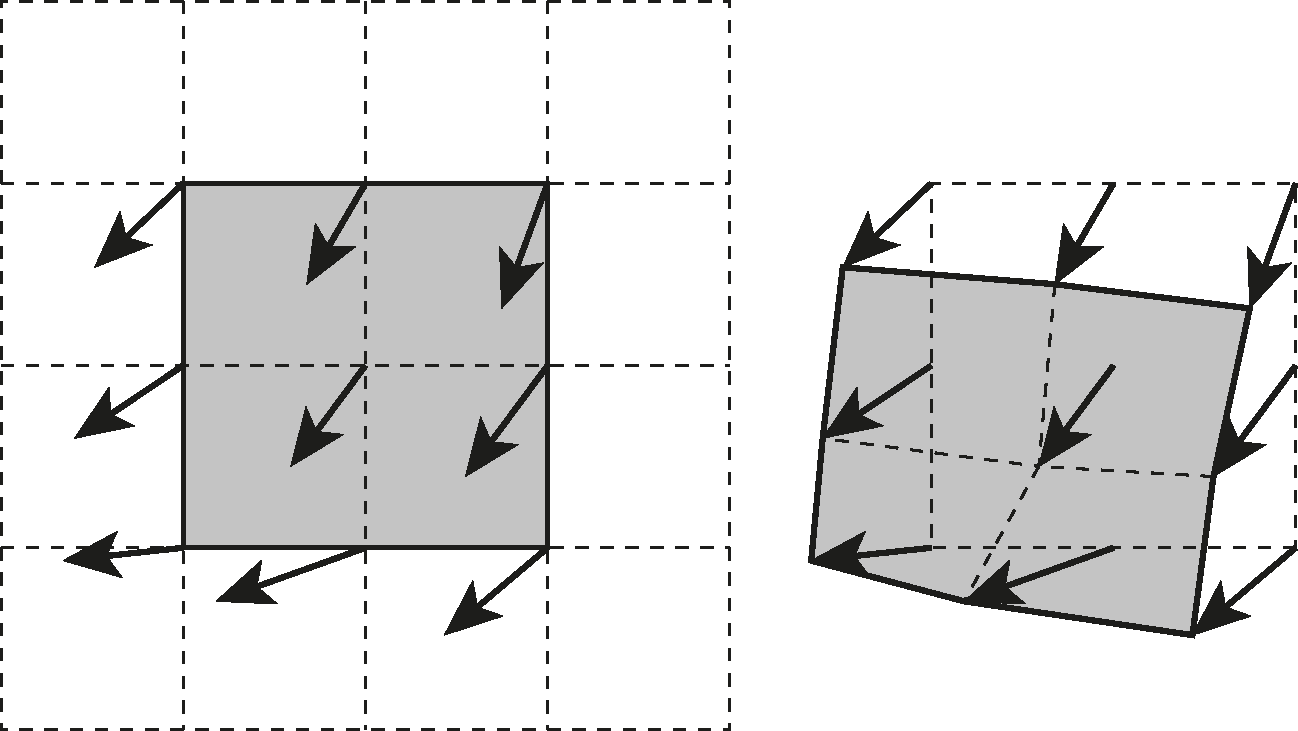
\includegraphics[width=8cm]{./2_DPIV/TehnikaDeformacijeProzora.pdf} 
	\caption{Princip tehnike deformacije prozora, na lijevoj slici se nakon prvog prolaza dobije informacija o pomaku koja je vidljiva na 9 lokacija. Informacije o pomacima se nakon toga interpoliraju kako bi se dobio pomak svakog pixela prozora ispitivanja, te konačno imamo novi prozor ispitivanja koji će se koristiti u sljedećem prolazu DFT-a \cite{thielicke2014_phd}}
	\label{Tehnika deformacije prozora}
\end{figure}
\FloatBarrier
\subsection{Računanje korelacijskog koeficijenta}
U brojnim slučajevima korisno je kvantificirati stupanj korelacije između dva uzorka prozora ispitivanja. Standardna kros-korelacijska funkcija (jednadžba \ref{eqn:2.4}) daje različite vrijednosti maksimalnih korelacija za isti stupanj poklapanja, zbog toga što kros-korelacijska funkcija nije normalizirana. Na primjer, prozori ispitivanja sa mnogo (svijetlih) čestica daju mnogo veću vrijednost korelacijskog koeficijenta od uzoraka gdje su čestice manje svijetle. Na ovaj način usporedba stupnja korelacije između individualnih prozora ispitivanja nije moguća. Funkcija kros-korelacijskog koeficijenta (\ref{eqn:2.6}) normalizira kros-korelacijsku funkciju (\ref{eqn:2.4}) na način:
\begin{subequations} \label{eqn:2.6}
	\begin{equation}
		c_{II}(x, y)=\frac{C_{II}(x, y)}{\sqrt{\sigma_{I}(x, y)}\sqrt{\sigma_{I'}(x, y)}} \tag{\ref{eqn:2.6}}
	\end{equation}
gdje su:
	\begin{align}
		\begin{split} \label{eqn:2.6a}
			C_{II}(x, y) &= \sum_{i=0}^{M}\sum_{j=0}^{N}\left[ I(i, j)-\mu_{I}\right]\left[ I'(i+x, j+y)-\mu_{I'}(x, y)\right]
		\end{split} \\
		\begin{split} \label{eqn:2.6b}
			\sigma_{I}(x, y) &= \sum_{i=0}^{M}\sum_{j=0}^{N}\left[I(i, j)-\mu_{I}\right]^{2}
		\end{split} \\
		\begin{split} \label{eqn:2.6c}
			\sigma_{I'}(x, y) &= \sum_{i=0}^{M}\sum_{j=0}^{N}\left[I'(i, j)-\mu_{I'}(x, y)\right]^{2}
		\end{split}
	\end{align}
\end{subequations}
Vrijednost $\mu_{I}$ je prosjek predloška prozora i računa se samo jednom, dok $\mu_{I'}(x, y)$ je prosjek $I'$ koji se podudara predloškom prozora $I$ na poziciji $(x, y)$. $I'$ mora se izračunati na svakoj poziciji $(x, y)$. Jednadžbu \ref{eqn:2.6} značajno je teže implementirati koristeći FFT algoritam i obično se računa direktno u prostornoj domeni. Unatoč računalnoj kompleksnosti, jednadžba dopušta da uzorci (prozori) budu nejednake veličine što može biti vrlo korisno u podudaranju malih grupa čestica. Ipak aproksimacija prvog reda pravilnoj normalizaciji je moguća ako su prozori ispitivanja jednake veličine i nisu obloženi nulama. 
\begin{enumerate}[label=\textbf{Korak \arabic*:}, leftmargin=*, align=left, topsep=0pt, itemsep=0em]
	\item Uzrokovati prozore ispitivanja na željenim lokacijama, te izračunati srednju i standardnu devijaciju svake slike
	\item Oduzeti srednju vrijednost od svakog uzorka
	\item Izračunati kros-korelacijsku funkciju koristeći 2D FFT-ove (kao što je prikazano na slici \ref{sl:2.10})
	\item Podijeliti kros-korelacijske vrijednosti sa standardnom devijacijom originalnog uzorka. Zbog postupka normalizacije rezultirajuće vrijednosti će upasti u raspon $-1\leq c\leq 1$.
	\item Nastaviti sa detekcijom korelacijskog vrha uzimajući u obzir sve (ne)mogućnosti FFT kros-korelacije.
\end{enumerate}
\subsection{Pronalazak korelacijskog vrha}
Još jedan veoma bitan faktor pri PIV analizi koji izravno utječe na točnost mjerenja je odabir tehnike pronalaska korelacijskog vrha. Cjelobrojni pomak dva prozora ispitivanja može biti izravno određen iz lokacije najvećeg vrha korelacije korelacijske matrice \cite{thielicke2014_article}. No, lokacija nadalje može biti određena i sub-pixelskom preciznošću koristeći razne metode.
\par
Kako su ulazni podaci u PIV analizi diskretizirani, vrijednosti korelacije postoje samo za integralne pomake. Najveća vrijednost korelacije tada bi omogućila određivanje pomaka sa nesigurnošću od $\pm \, 1/2$ pixela. Međutim, kako je kros-korelacijska funkcija statistička mjera najboljeg poklapanja, korelacije vrijednosti oko vrha također sadrže korisne informacije \cite{raffel2018_book}. Na primjer, ako ispitivani uzorak sadrži $10$ parova čestica koje su dale procijenjeni pomak koji u prosjeku malo varira sa vrijednosti od $2.5$ pixela, statistički bi to značilo da je $5$ parova čestica dalo pomak od $3$ pixela, a preostalih $5$ parova pomak od $2$ pixela. Iz ovog grubog primjera, jasno je kako se informacije skrivene u vrijednostima korelacije mogu iskoristiti za procjenu srednjeg pomaka slike unutar prozora ispitivanja.
\par
U literaturi \cite{raffel2018_book} opisane su razne metode procjene lokacije korelacijskog vrha. Jedan od robustnijih načina procjene lokacije je taj da se korelacijski podaci aproksimiraju sa određenom funkcijom. Ova metoda je posebno dobra kod uskih korelacijskih vrhova, pošto se ovim pristupom uobičajeno koriste samo 3 susjedne vrijednosti korelacijske matrice (u x ili y smjeru). Najčešće korištena je aproksimacija vrha korelacije Gauss-ovom funkcijom. 
\begin{equation}
	f(x)=C\exp \left[\dfrac{-(x_{0}-x)^{2}}{k}\right]
	\label{eqn:2.7}
\end{equation}
Korištenje Gauss-ove funkcije za aproksimaciju je najprikladnije iz razloga što individualne snimke čestica usko se podudaraju sa Gauss-ovom distribucijom intenziteta (imaju oblik Airy-eve funkcije intenziteta - \textit{Slika \ref{sl:3.2}}), te kros-korelacija dvije Gauss-ove distribucije ponovno daje korelacijsku matrica sa Gauss-ovom distribucijom.
\par
Kada je poznata najveća vrijednost vrha korelacije u korelacijskoj matrici, pomoću ostalih podataka iz matrice Gauss-ovom funkcijom moguće je točnije (sub-pixelski) aproksimirati vrh korelacije (\textit{Slika \ref{sl:2.12}}). Dovoljna je upotreba samo neposredno susjednih vertikalnih i horizontalnih pixela, te je moguće evaluirati x i y os odvojeno. Implementacija aproksimacije u 3 točke se vrši na način:
\begin{figure}[h]  
	\centering
	%\usepackage{graphicx}
	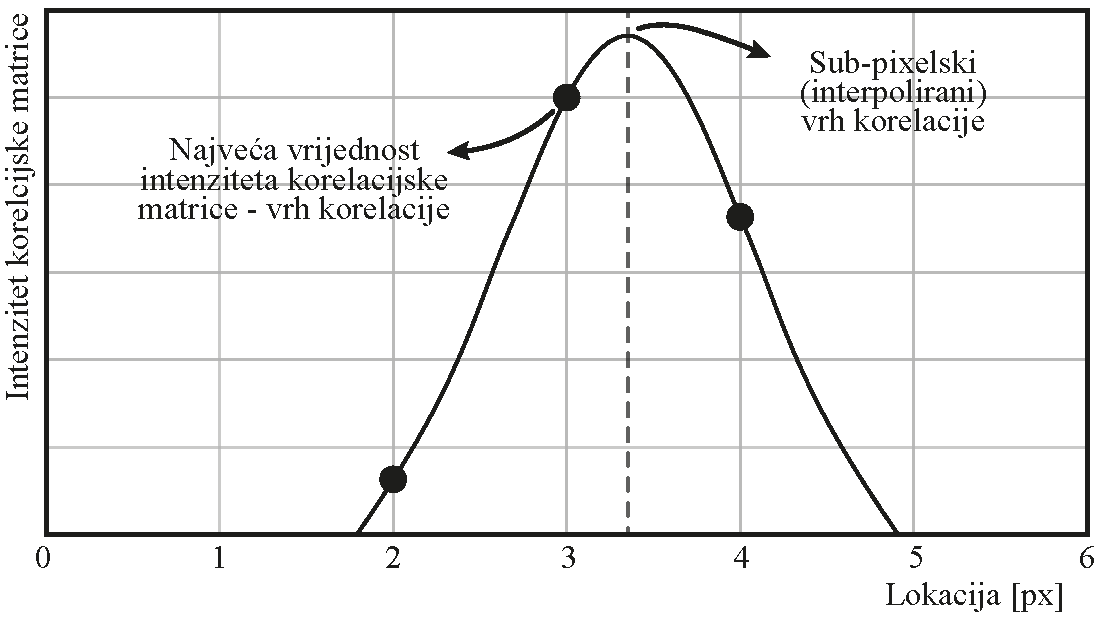
\includegraphics[width=11cm]{./2_DPIV/2_12DetekcijaVrha.pdf} 
	\caption{Princip aproksimacije u 3 točke Gauss-ovom funkcijom, točke predstavljaju vrijednosti intenziteta korelacijske matrice za samo jednu os}
	\label{sl:2.12}
\end{figure}
\begin{enumerate}[label=\textbf{Korak \arabic*:}, leftmargin=*, align=left, topsep=0pt, itemsep=0em]
	\item Pronaći maksimalne korelacijske vrijednosti $R(i, j)$ u korelacijsku ravninu $R_{II}$, te zapamtiti njihove $(i, j)$ koordinate.
	\item Izvući četiri susjedne korelacijske vrijednosti: $R_{(i-1,j)}$, $R_{(i+1,j)}$, $R_{(i,j-1)}$ i $R_{(i,j+1)}$
	\item Koristeći tri točke u svakom smjeru osi, provući Gauss-ovu krivulju gdje su $C$, $x_{0}$ i $k$ koeficijenti koje treba dobiti nekom od metoda interpolacije (npr. nelinearna regresija iz jednadžbe \ref{eqn:2.7})
\end{enumerate}
Potrebno je napomenuti u slučaju da je pomak čestica unutar prozora ispitivanja podvrgnut smicanju ili rotaciju ili su snimke previše mutne tada korelacijski vrh ima ne-simetričan (eliptičan) oblik, te korištenje aproksimacije u jednom smjeru sa 3 vrijednosti Gauss-ovom funkcijom može izazvati pogreške. Ovaj efekt se može izbjeći ako se koristi 2D aproksimacija Gauss-ovom funkcijom (fittanje u 9 točaka).
\begin{equation}
	f(x, y)=I_{0}\, \exp \left[\dfrac{-(x-x_{0})^{2}}{(1/8)d_{\tau x}^{2}}-\dfrac{-(y-y_{0})^{2}}{(1/8)d_{\tau y}^{2}}-\dfrac{k_{xy}(x-x_{0})(y-y_{0})}{d_{\tau x}d_{\tau y}}\right]
	\label{eqn:2.8}
\end{equation}
Jednadžba \ref{eqn:2.8} sadrži ukupno 6 koeficijenata koje je potrebno dobiti (naprimjer ponovno nekom regresijskom metodom). Koeficijenti $d_{\tau x}$ i $d_{\tau y}$ predstavljaju širine korelacijskih vrhova u $x$ i $y$ smjeru, dok koeficijent $k_{xy}$ predstavlja "eliptičnost" korelacijskog vrha. Maksimalni iznos vrha korelacije $I_{0}$ određen je pozicijom $x_{0}$ i $y_{0}$.
\FloatBarrier
\section{Postprocesiranje PIV podataka}
Iako napredni kros-korelacijski algoritam pruža dosta robusnu procjenu brzine unutar područja ispitivanja, i dalje mnogi faktori (loše osvjetljenje, jako 3D strujanje,...) uzrokuju nepravilnu korelaciju koju je do određene mjere naknadno moguće ispraviti koristeći razne tehnike obrade dobivenih PIV rezultata. U principu, post-procesiranje PIV podataka sastoji se od sljedećih koraka:
\begin{description}[style=unboxed,leftmargin=0cm]
	\item[Provjera valjanosti neobrađenih (\textit{eng. raw}) podataka.] Nakon automatske evaluacije PIV snimki, određeni broj očito nepravilno određenih vektora brzina koji se na engleskom nazivaju "\textit{outliers}" ("\textit{vrijednosti koje strše}") obično se može prepoznati vizualnom inspekcijom neobrađenih podataka. U svrhu da se odrede nepravilni vektori ovaj post-proces prepoznavanja pogrešnih vektora mora biti automatiziran. Potrebno je napomenuti kako je provjera valjanosti podataka prvi i najvažniji korak, jer utječe na kvalitetu provedbe svih ostalih tehnika postprocesiranja PIV podataka.
	\item[Zamjena pogrešnih podataka.] Kod većine post-proces algoritama potrebno je imati kompletno popunjena polja podataka u Kartezijevoj mreži, što je i slučaj kod numeričkih simulacija. Ako se dogodi da nedostaje jedan podatak u mreži, taj podatak je potrebno aproksimirati sa određenom vrijednosti brzine.
	\item[Smanjenje podataka.] Često je komplicirano pratiti nekoliko tisuća podataka o brzinama i pomacima, pogotovo u slučaju 3D PIV analize i dugotrajnih strujanja. Usrednjavanje podataka u ovim slučajevima je poprilično jednostavna tehnika. U slučaju da je uzorkovanje strujanja više-manje uvjetovano, te tada treba razlikovati periodične i ne-periodične fluktuacije u strujanju, smanjivanje podataka usrednjavanjem više nije tako jednostavno. Također moguće je podatke o strujanju pojednostavniti uz pomoć operatora za vektorsko polje (npr. korištenje rotacije i divergencije brzine). Nadalje u novije vrijeme evaluacija nestacionarnih strujanja zahtjeva pojednostavljenja koja se izvršavaju preko dekompozicijskih tehnika. Najčešće korištene dekompozicijske tehnike u ovom slučaju su: \textit{pravilna ortogonalna dekompozicija} (POD) (\textit{eng. Proper Orthogonal Decomposition}) poznata kao i \textit{analiza glavnih komponenti} (PCA) (\textit{eng. Principal Component Analysis}), te \textit{dinamička modalna dekompozicija} (DMD) (\textit{eng. Dynamic Mode Decomposition}).
	\item[Asimilacija podataka] Često kada se provode PIV eksperimenti, dosta stvari o promatranoj vrsti strujanja je poznato i analitički određeno, pogotovo za slučajeve elementarnih tipova strujanja. U tom slučaju PIV podatke je moguće obraditi na takav način da lokalno ispunjavaju matematičke zakone.
\end{description}
\subsection{Provjera valjanosti podataka}
Kako je broj nepravilnih vektora brzina znatan, čak i ako se koriste najnaprednije korelacijske metode. Potrebno je korištenje (polu)automatske provjere valjanosti podataka (\textit{eng. Data Validation}) kako bi se učinkovito suzbili pogrešni podaci. U literaturama postoji mnogo metoda i algoritama za provjeru valjanosti podataka, te treba napomenuti kako nijedna od tih tehnika nije generalno dobra za sve PIV analize. No, ipak u ovom radu će biti opisane neke od najkorištenijih metoda provjere valjanosti podataka, koje su i implementirane u korišteni softver.
\par
Prije samog opisa validacijskih algoritama, potrebno je definirati varijable i izraze koji će se koristiti u daljnjem tekstu \cite{raffel2018_book}. Neka je trenutno polje brzina $(U, V)$ uzorkovano ("ispitano") na lokacijama koje formiraju strukturiranu mrežu u polju strujanja.  U ovom slučaju mreža  je prikazana na \textit{Slici \ref{sl:2.13}} i sastoji se od $I\times J$ čvorova, međusobno udaljenih u $X$ i $Y$ smjeru za $\Delta X$ i $\Delta Y$. U svakom čvoru $i, j \, (i=1,\dots ,I;\, j=,\dots ,J)$ opisana je brzina $\boldsymbol{U}_{2D}(i, j)$. U ovom slučaju bitna je veza između $\boldsymbol{U}_{2D}(i, j)$ i njegovih najbližih susjeda koji su označeni sa $\boldsymbol{U}_{2D}(n)$ gdje $n$ ide $n \, (n=1,\dots,N)$, a $N$ označava broj susjeda kojih je uobičajeno osam. Sada je potrebno definirati vrijednost razlike vektora između središnjeg vektora $\boldsymbol{U}_{2D}(i, j)$, te susjednih vektora $\boldsymbol{U}_{2D}(n)$:
\begin{equation}
	|\boldsymbol{U}_{\Delta , n}|=|\boldsymbol{U}_{2D}(n)-\boldsymbol{U}_{2D}(i,j)|
	\label{eqn:2.9}
\end{equation}
\begin{figure}[h]  
	\centering
	%\usepackage{graphicx}
	\includegraphics[width=12cm]{./2_DPIV/2_13MeshPostProc.pdf} 
	\caption{Shema mreže podataka sa označenim vektorima}
	\label{sl:2.13}
\end{figure}
\begin{description}[style=unboxed,leftmargin=0cm]
	\item[Provjera razlike vektora] Jednostavna tehnika za suzbijanje nepravilnih vektora je definiranje granice vrijednosti komponenti vektora brzina za određeno područje, tvz. gradijent filtar. Gradijent filtar se računa uz pomoć izraza \ref{eqn:2.9}. Ideja korištenja gradijent filtra je u tome da se odredi broj instanci za koje je izraz $|\boldsymbol{U}_{\Delta, n}|< \epsilon_{grani\textup{č}ni}$ prekršen. U slučaju da je vektor pomaka različit od polovine svojih susjeda, taj vektor bi trebao biti ispravljen. Ova provjera dodatno može biti modificirana na način da se odrede $U$ i $V$ komponente brzine za svaki čvor, te na taj način vrši sofisticiranija provjera u koju se mogu uključiti i donja i gornja granica.  Nedostatak ove metode je u tome što se temelji na prijašnjem iskustvu, te pretpostavci i znanju osobe koja provodi eksperiment, što unosi subjektivno mišljenje u mjerenje. Također, donja i gornja granice brzine ($t_{d}$ i $t_{g}$) se mogu odrediti (polu)automatski uz pomoć prosječne vrijednosti i standardne devijacije brzine u određenom području, te taj način vrši se dinamička provjera razlike vektora \cite{thielicke2014_phd}:
	\begin{equation}
		t_{d}=\bar{\boldsymbol{U}}_{2D}-n \, \sigma_{\boldsymbol{U}_{2D}}
		\label{eqn:2.10}
	\end{equation}
	\begin{equation}
		t_{g}=\bar{\boldsymbol{U}}_{2D}+n \, \sigma_{\boldsymbol{U}_{2D}}
		\label{eqn:2.11}
	\end{equation}
	gdje je $\bar{\boldsymbol{U}}_{2D}$ prosječna brzina, a $\sigma_{\boldsymbol{U}_{2D}}$ standardna devijacija brzine $\boldsymbol{U}_{2D}$. Dok $n$ predstavlja varijablu kojom korisnik definira strogoću filtra brzina. U praksi ovaj filtar dosta efikasno funkcionira jer se prilagođava prirodi strujanja. U turbulentnim strujanjima, vrijednost standardne devijacije je visoka, pa puno vektora prođe kroz filtar, dok kod laminarnih strujanja, standardna devijacija ima nisku vrijednost, te će filtar izbaciti vektore koji malo odstupaju od prosjeka.
	\item[Medijan test] Medijansko filtriranje je često korištena tehnika u obradi slike kojom se uklanja lažni šum. U PIV analizi isto tako može efikasno poslužiti u uklanjanju nepravilnih vektora brzina. Medijansko filtriranje zahtjeva da se svi susjedni vektori $\boldsymbol{U}_{2D}(n)$ uzlazno sortiraju (ili po njihovoj veličini ili po veličini njihovih $U$ i $V$ komponenti). Središnja vrijednost sortiranih vrijednosti u tom slučaju predstavlja medijan, te se središnji vektor $\boldsymbol{U}_{2D}(i,j)$ testira izrazom:
	\begin{equation}
		|\boldsymbol{U}_{2D}(med)-\boldsymbol{U}_{2D}(i,j)|<\epsilon_{grani\textup{č}ni}
		\label{eqn:2.12}
	\end{equation}
	\item[Normalizirani medijan test] Neznatna modifikacija medijan filtriranja predložena je u literaturi \cite{westerweel2005}, te implementirana u PIVlab softver. Normalizacija jednadžbe za standardni medijanski test \ref{eqn:2.12} daje prilično univerzalnu funkciju gustoće vjerojatnosti (PDF) za ostatak tako da jedinstvena granična vrijednost može biti primijenjena da efektno detektira nepravilne vektore. Normalizacija zahtjeva da ostatak (\textit{eng. residual}) $r_{i}=|\boldsymbol{U}_{i}-\boldsymbol{U}_{med}|$ bude prvo određen za svaki susjedni vektor $\{\boldsymbol{U}_{i}\, |\, i=1,\dots,8\}$. Nakon toga odredi se medijan svih dobivenih osam ostataka $r_{med}$, te se koristi kao normalizacija standardnog medijanskog testa:
	\begin{equation}
		\dfrac{|\boldsymbol{U}_{2D}(med)-\boldsymbol{U}_{2D}(i,j)|}{r_{med}+\epsilon_{0}}<\epsilon_{grani\textup{č}ni}
		\label{eqn:2.13}
	\end{equation}
	Dodatni član $\epsilon_{0}$ u jednadžbi \ref{eqn:2.13} dodan je kako bi se u obzir uzele preostale fluktuacije dobivene korelacijskom analizom inače mirnog ili homogenog strujanja. U praksi $\epsilon_{0}$ se uobičajeno postavlja na vrijednost od $0.1$ - $0.2$ pixela, što odgovora srednjoj vrijednosti šuma u PIV podacima. Univerzalnost opisanog testa demonstrirana je u literaturi \cite{westerweel2005} i pokazano je kako se ovom metodom pokriva širok raspon strujanja pri različitim Reynolds-ovim brojevima.
	\item[Provjera vektora brzina bazirana na pravilnoj ortogonalnoj dekompoziciji - POD] Korištenje POD-a  u svrhu provjere PIV podataka bazira se na pretpostavci da nepravilni vektori nisu korelirani sa određenom značajkom strujanja, to jest da je pojava nepravilnih vektora striktno nasumični efekt \cite{raffel2018_book}. Jednom kada je set podataka rastavljen u svoje ortogonalne modove. Najveće rangirani mod predstavlja dominantnu fizičku fluktuaciju brzine. Energija sadržana u modovima najnižeg ranga uglavnom predstavlja nasumične greške i nepravilne vektore. Nakon POD dekompozicije seta podataka, vrši se rekonstrukcija niskog reda (bazirana naprimjer na $95\%$ ukupne energije) koja je robusna tehnika eliminiranja nepravilnih vektora i istodobnog mijenjanja istih realnim procjenama.
\end{description}
\subsection{Sheme zamjene i zaglađivanja podataka}
Nakon provjere svih podataka, obično se popunjavanje i zamjena vektora koji nedostaju vrši bilinearnom interpolacijom. Prema literaturi \cite{westerweel1994efficient} vjerojatnost da se jedan nepravilni vektor nalazi u susjedstvu drugog susjednog vektora dana je sa binominalnom distribucijom. Naprimjer, ako podaci sadrže $5\%$ nepravilnih vektora, onda više od $80\%$ podataka može biti ispravljeno sa ravnom bilinearnom interpolacijom. Preostali podaci koji nedostaju mogu biti popunjeni nekom od vrsta težinskog usrednjavanja okolnih podataka \cite{raffel2018_book}.
\par
PIVlab softver koristi solver granične vrijednosti (\textit{eng. boundary value solver}) za interpolaciju podataka, koji je originalno razvijen za rekonstrukciju slika kojima nedostaju određene informacije. Ovim pristupom omogućena je generalno glatka interpolacija, te kod interpolacije područja gdje je nedostaje veća količina podataka, podaci teže ka srednjaku graničnih brzina.
\par
U literaturi \cite{thielicke2014_phd} prikazano je kako razne tehnike interpolacije djeluju na PIV podatke. Najjednostavnija interpolacijska shema, obično usrednjavanje podataka sa $3 \times 3$ kernelom daje najlošije rezultate (\textit{Slika \ref{sl:2.14}}). 2D spline interpolacija daje dobre rezultate ako je količina podataka kojih nedostaju ispod $5\%$. U slučaju da nedostaje više od $5\%$ vektora, onda postoji i veća vjerojatnost povezanosti podataka koji nedostaju, tada \textit{Spline interpolacije} daju značajno lošije rezultate od \textit{Solver graničnih vrijednosti}, zbog toga što spline sa premalo čvorova jako lako "prebaci" nivo interpolacije (\textit{eng. overshoot}).
\par
Također, neke PIV post-procesorske metode zahtijevaju zaglađivanje podataka. Razlog tome je što za razliku od podataka dobivenih numeričkim simulacijama, podaci dobiveni eksperimentalno gotovo uvijek imaju šum. Rješavanje problema šuma unutar podataka najčešće se radi korištenjem $2 \times 2$, $3 \times 3$, ili većeg kernela za zaglađivanje koji se konvoluira za podacima. Odabir kernela bi svakako trebao biti takav da kernel filtar bude manji od veličine prozora ispitivanja, kako bi se efekt nisko-propusnog filtriranja podataka o polju brzina sveo na minimum. Kernel matrice mogu imati koeficijente u obliku srednjih ili medijanskih vrijednosti.
\begin{figure}[h]  
	\centering
	%\usepackage{graphicx}
	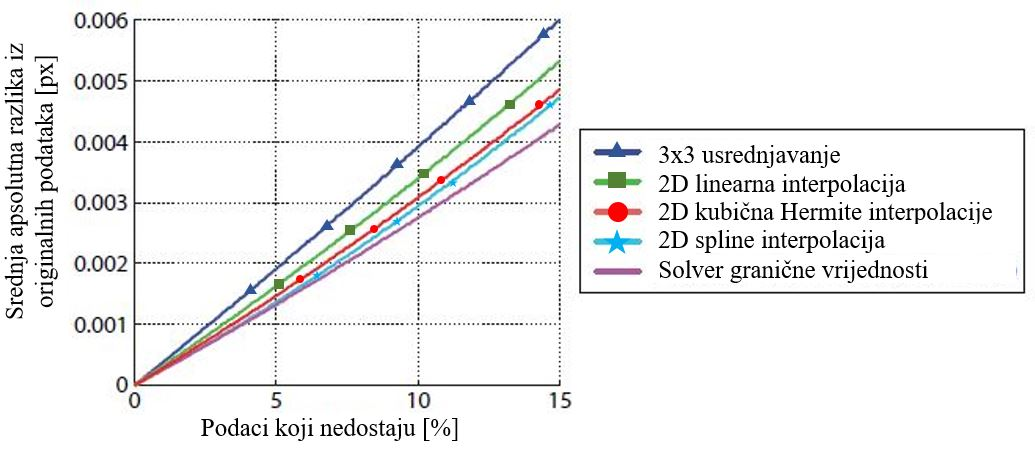
\includegraphics[width=14cm]{./2_DPIV/2_14PrefInterpolacije.jpg} 
	\caption{Performanse najčešće korištenih interpolacijskih shema. Solver granične vrijednosti ima najbolje rezultate za za PIV mjerenja gdje nedostaje mnogo podatka ($>10\%$) \cite{thielicke2014_phd}}
	\label{sl:2.14}
\end{figure}
\par
U novije vrijeme razvijen je napredniji algoritam zaglađivanja podataka koji se naziva "\textit{Smoothn}" \cite{garcia2010robust}, te je baziran na penalizirajućoj metodi najmanjih kvadrata. Na \textit{Slici \ref{sl:2.15}} prikazana je prosječna i maksimalna apsolutna razlika između točnih i izračunatih vrijednosti kod korištenja tri algoritma za zaglađivanje, te kod podataka koji nisu podvrgnuti niti jednom algoritmu za zaglađivanje. Sa slike je vidljivo kako korištenje algoritma daje podatke koji imaju mnogo manje šuma, te samim time povećavana je kvaliteta procjene brzine.
U PIVlab softver implementiran je "Smoothn" algoritam.
\begin{figure}[h]  
	\centering
	%\usepackage{graphicx}
	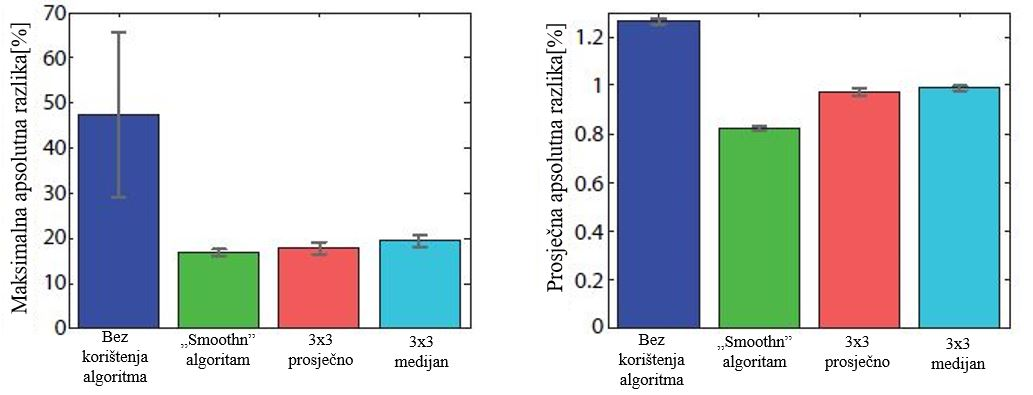
\includegraphics[width=16cm]{./2_DPIV/2_15AlgoritmiZaZagladivanje.jpg} 
	\caption{Validacija algoritama za zaglađivanje. Usporedba između maksimalnih i prosječnih izračunatih brzina i točnih podataka \cite{thielicke2014_phd}.}
	\label{sl:2.15}
\end{figure}
\FloatBarrier
\subsection{Korištenje vektorskih operatora}
Mnoga promatrana strujanja otkrivaju kompleksne uzorke koje je teško opisati samo sa mapom polja brzina, stoga ako ja moguće dobivene PIV podatke treba dalje obraditi i pojednostavniti. Nadalje, informacije o brzini često nisu glavni fizički interes strujanja, nego da bi strujanje bilo do kraja razriješeno potrebno je saznati informacije o polju tlakova i gustoća, jer to su preostali članovi Navier-Stokesove jednadžbe kojom se opisuje ponašanja fluida:
\begin{equation}
	\rho \dfrac{\mathrm{D}\boldsymbol{U}}{\mathrm{D}t}=-\nabla p+ \mu \nabla^{2}\boldsymbol{U}+\boldsymbol{f}
	\label{eqn:2.14}
\end{equation}
gdje $\boldsymbol{f}$ predstavlja doprinos masenih sila (npr. gravitacija). Načini na koji se dobivaju tlak i gustoća predmet je najnovijih PIV istraživanja i tehnologija (tomografski PIV, Shake-The-Box PIV,...). No ipak, 2D PIV i sam omogućava procjenu drugih fizički relevantnih veličina postupcima diferencijacije i integracije.
\par
Kod diferencijacije poseban interes ima polje vrtloga (rotacije) zbog toga što ova veličina, za razliku od polja brzina je neovisna o referentnom okviru. Posebno, ako je vremenski razriješeno, polje vrtloga može biti mnogo više korisno u proučavanju strujanja, pogotovo u strujanjima gdje ima mnogo vrtloga i turbulencija. Za nestlačivo strujanje ($\nabla \cdot \boldsymbol{U}=0$) Navier-Stokesova jednadžba može se zapisati pod uvjetima vrtloženja:
\begin{equation}
	\dfrac{\partial \boldsymbol{\omega}}{\partial t}+\boldsymbol{U}\cdot\nabla\boldsymbol{\omega}=\boldsymbol{\omega}\cdot\nabla\boldsymbol{U}+\nu\nabla^{2}\boldsymbol{\omega}
	\label{eqn:2.15}
\end{equation}
gdje se opisuje stopa promjene vrtloženja fluidnog elementa. U jednadžbi \ref{eqn:2.15} radi jednostavnosti izostavljen je član koji opisuje masene sile ($\boldsymbol{f}=0$), te se može primijetiti kako više nema člana koji opisuje tlak. No ipak usprkos prikazanim pojednostavljenjima posljednji član $\nabla^{2}\boldsymbol{\omega}$ i dalje je teško odrediti iz PIV podataka.
\subsection{Procjena diferencijalnih veličina}
Prije samog računanja diferencijalnih veličina iz polja podataka o brzinama treba odrediti koje se sve veličine uopće mogu izvući iz ravninskog polja brzina. Standardni 2D PIV naravno omogućuje samo dvo-komponentno polje brzina (zanemarena činjenica da 2D PIV daje 2D projekciju 3D vektora), dok je sa ostalim nadogradnjama PIV tehnologije (npr. stereoskopski PIV, tomografski PIV,...) moguće dobiti i polje brzina sa sve tri komponente. Za početak, kod 2D PIV mjerenja iz samo jednom snimane laserske ravnine (isključeno računanje gradijenata brzine u smjeru normalnom na ravninu) dan je izraz za tenzor promjene brzine (ili tenzor deformacija) $\mathrm{d}\boldsymbol{U}/\mathrm{d}\boldsymbol{X}$:
\begin{subequations}\label{eqn:2.16}
	\begin{equation}
		\dfrac{\mathrm{d}\boldsymbol{U}}{\mathrm{d}\boldsymbol{X}} = 
		\begin{bmatrix}
			\dfrac{\partial U}{\partial X}       &   \dfrac{\partial V}{\partial X}       &   \dfrac{\partial W}{\partial X}       \\
			\dfrac{\partial U}{\partial Y}       &   \dfrac{\partial V}{\partial Y}       &   \dfrac{\partial W}{\partial Y}       \\   
			\dfrac{\partial U}{\partial Z}       &   \dfrac{\partial V}{\partial Z}       &   \dfrac{\partial W}{\partial Z}       \\
		\end{bmatrix}
	\tag{\ref{eqn:2.16}}
	\end{equation}
	Tenzor deformacija može se raščlaniti na svoj simetrični i antisimetrični dio:
	\begin{align}\label{eqn:2.16a}
		\dfrac{\mathrm{d}\boldsymbol{U}}{\mathrm{d}\boldsymbol{X}} = 
		&\underbrace{\begin{bmatrix}
				\dfrac{\partial U}{\partial X}       &   \dfrac{1}{2}\left(\dfrac{\partial V}{\partial X}+\dfrac{\partial U}{\partial Y}\right)       &   \dfrac{1}{2}\left(\dfrac{\partial W}{\partial X}+\dfrac{\partial U}{\partial Z}\right)       \\
				\dfrac{1}{2}\left(\dfrac{\partial U}{\partial Y}+\dfrac{\partial V}{\partial X}\right)       &   \dfrac{\partial V}{\partial Y}       &   \dfrac{1}{2}\left(\dfrac{\partial W}{\partial Y}+\dfrac{\partial V}{\partial Z}\right)       \\   
				\dfrac{1}{2}\left(\dfrac{\partial U}{\partial Z}+\dfrac{\partial W}{\partial X}\right)       &   \dfrac{1}{2}\left(\dfrac{\partial V}{\partial Z}+\dfrac{\partial W}{\partial Y}\right)       &   \dfrac{\partial W}{\partial Z}       \\
		\end{bmatrix}}_{\text{simetr.}} \notag \\
		&+ \underbrace{\begin{bmatrix}
				0       &   \dfrac{1}{2}\left(\dfrac{\partial V}{\partial X}-\dfrac{\partial U}{\partial Y}\right)       &   \dfrac{1}{2}\left(\dfrac{\partial W}{\partial X}-\dfrac{\partial U}{\partial Z}\right)       \\
				\dfrac{1}{2}\left(\dfrac{\partial U}{\partial Y}-\dfrac{\partial V}{\partial X}\right)       &   0       &   \dfrac{1}{2}\left(\dfrac{\partial W}{\partial Y}-\dfrac{\partial V}{\partial Z}\right)       \\   
				\dfrac{1}{2}\left(\dfrac{\partial U}{\partial Z}-\dfrac{\partial W}{\partial X}\right)       &   \dfrac{1}{2}\left(\dfrac{\partial V}{\partial Z}-\dfrac{\partial W}{\partial Y}\right)       &   0       \\
		\end{bmatrix}}_{\text{antisimetr.}}
	\end{align}
\end{subequations}
Ako članove u jednadžbi \ref{eqn:2.16a} zamijenimo sa komponentama deformacije i rotacije jednadžba ima oblik:
\begin{equation}
	\dfrac{\mathrm{d}\boldsymbol{U}}{\mathrm{d}\boldsymbol{X}} = 
	\underbrace{\begin{bmatrix}
			\epsilon_{XX}       &   \dfrac{1}{2}\epsilon_{XY}       &   \dfrac{1}{2}\epsilon_{XZ}       \\
			\dfrac{1}{2}\epsilon_{YX}       &   \epsilon_{YY}       &   \dfrac{1}{2}\epsilon_{YZ}       \\   
			\dfrac{1}{2}\epsilon_{ZX}       &   \dfrac{1}{2}\epsilon_{ZY}       &   \epsilon_{ZZ}       \\
	\end{bmatrix}}_{\text{matrica brzina deformacije}} + 
	\underbrace{\begin{bmatrix}
			0       &   \dfrac{1}{2}\omega_{Z}       &   -\dfrac{1}{2}\omega_{X}       \\
			-\dfrac{1}{2}\omega_{Z}       &   0       &   \dfrac{1}{2}\omega_{Y}       \\   
			-\dfrac{1}{2}\omega_{X}       &   \dfrac{1}{2}\omega_{Y}       &   0       \\
	\end{bmatrix}}_{\text{matrica rotacije}}
	\label{eqn:2.17}
\end{equation}
gdje dijagonalni članovi matrice brzine deformacije predstavljaju deformaciju zbog produljenja, a van-dijagonalni članovi predstavljaju deformaciju zbog smicanja, dok svi članovi matrice rotacije predstavljaju komponente rotacije.
\par
Kako konvencionalni 2D PIV omogućava samo $U$ i $V$ komponente brzine, te samim time svi podaci mogu se diferencirati samo u $X$ i $Y$ smjeru, samo se nekoliko članova tenzora deformacije $\mathrm{d}\boldsymbol{U}/\mathrm{d}\boldsymbol{X}$ može procijeniti sa PIV podacima. Najčešći parametri korišteni za vizualizaciju gradijenata u strujanju prikazani su u \textit{Tablici \ref{tab:2.2}}. Ovi parametri su izračunati uz pomoć lokalne stope promjene brzine (derivacije brzine).
\begin{table}[h]
	\centering
	\caption{Gradijentni parametri koji se mogu izvesti iz informacija o brzinama strujanja dobivenih putem 2D-PIV, te dodatno pomoći pri interpretaciji promatranog strujanja \cite{stamhuis2006basics}}
	\resizebox{\textwidth}{!}{%
	\begin{tabular}{cll}
		\hline
		\rowcolor[HTML]{9B9B9B} 
		\textbf{Parametar}                                                              & \textbf{Predstavlja:}                                                                                                                               & \textbf{Jednadžba}                                                                          \\ \hline
		\begin{tabular}[c]{@{}c@{}}Vrtložnost\\ (\textit{eng.vorticity})\end{tabular}            & \begin{tabular}[c]{@{}l@{}}Rotaciju fluida\\ ("komponenta rotacije normalna na lasersku ravninu")\end{tabular}                                      & $\omega_{Z}=\dfrac{\partial V}{\partial X}-\dfrac{\partial U}{\partial Y}$                  \\ \hline
		\begin{tabular}[c]{@{}c@{}}Stopa smicanja\\ (\textit{eng. shear rate})\end{tabular}      & \begin{tabular}[c]{@{}l@{}}Jačinu gradijenta brzine okomito na lokalnu brzinu\\ ("unutar-ravninsko klizanje susjednih slojeva fluida")\end{tabular} & $\epsilon_{XY}=\dfrac{\partial U}{\partial Y}+\dfrac{\partial V}{\partial X}$               \\ \hline
		\begin{tabular}[c]{@{}c@{}}Stopa istezanja\\ (\textit{eng. strain rate})\end{tabular}    & \begin{tabular}[c]{@{}l@{}}Jačina gradijenta brzine u smjeru lokalne brzine\\ ("unutar-ravninsko ubrzanje unutar jednog sloja fluida")\end{tabular} & $\epsilon_{XX}-\epsilon_{YY}=\dfrac{\partial U}{\partial X}-\dfrac{\partial V}{\partial Y}$ \\ \hline
		Divergenca                                                                      & \begin{tabular}[c]{@{}l@{}}Jačina izvan-ravninske stope strujanja\\ ("struja koja napušta i ulazi u lasersku ravninu")\end{tabular}                 & $\eta=\epsilon_{XX}+\epsilon_{YY}=\dfrac{\partial U}{\partial X}+\dfrac{\partial V}{\partial Y}$ \\ \hline
		\begin{tabular}[c]{@{}c@{}}Lokator vrtloga\\ (\textit{eng. vortex locator})\end{tabular} & \begin{tabular}[c]{@{}l@{}}Pronalazi centar vrtloga\\ (preko diskriminante za  kompleksne svojstvene vrijednosti)\end{tabular}                      &                                                                                             \\ \hline
	\end{tabular}}
\label{tab:2.2}
\end{table}
\par
Samo komponenta rotacije normalna na lasersku ravninu $\omega_{Z}$ može biti određena, zajedno sa unutar-ravninskim smicanjem $\epsilon_{XY}$ i divergencom $\eta$. Zanimljivo je napomenuti kako postojanje treće komponente brzine $W$, koja se dobije sa naprimjer stereoskopskim PIV mjerenjem ne daje nikakve dodatne komponente deformacije ili rotacije. Ako se pretpostavi nestlačivo strujanje ($\nabla \cdot \boldsymbol{U}=0$), suma unutar-ravninskih deformacija u jednadžbi za $\eta$ iz \textit{Tablice \ref{tab:2.2}} može biti iskorištena za procjenu izvan-ravninskog strujanja $\epsilon_{ZZ}$:
\begin{equation*}
	\epsilon_{ZZ}=\dfrac{\partial W}{\partial Z}=-\dfrac{\partial U}{\partial X}-\dfrac{\partial V}{\partial Y}=-\eta
\end{equation*}
Međutim potrebno je napomenuti kako veličina $\eta$ samo upućuje na prisutnost izvan-ravninskog strujanja, ali ne daje nikakve informacije o van-ravninskoj brzini $W$.
\FloatBarrier
\subsection{Procjena integralnih veličina}
\begin{description}[style=unboxed,leftmargin=0cm]
	\item[Linijski integral - Cirukulacija] Po definiciji, vrtloženje integrirano nad područjem $A$ jednako je cirkulaciji $\Gamma$. Stokesov teorem daje vezu između vrtloženja i cirkulacije, te uz pomoć njega operacija integriranja se reducira na linijski integral skalarnog produkta između lokalnog vektora brzine $\boldsymbol{U}$ i djelića elementa putanje vektora $d\boldsymbol{X}$, gdje je putanja integracije određena granicom $C$ zatvorenog područja $A$:
	\begin{align}
		\begin{split} \label{eqn:2.18}
			\Gamma&=\int_{A}\omega \, dA
		\end{split} \\
		\begin{split} \label{eqn:2.19}
			&=\oint_{C}\boldsymbol{U}\cdot d\boldsymbol{X}
		\end{split}
	\end{align}
	Za dvo-komponentne PIV podatke o brzinama u $XY$ ravnini sa $\boldsymbol{U}\, =\, (U,V)$, gornja jednadžba se svede na:
	\begin{align}
		\begin{split} \label{eqn:2.20}
			\Gamma&=\int \int_{A(X,Y)}\omega_{Z}\, dX \, dY
		\end{split} \\
		\begin{split} \label{eqn:2.21}
			&=\oint_{C(X,Y)}\boldsymbol{U}(\boldsymbol{X}, \boldsymbol{Y})\cdot d\boldsymbol{X}
		\end{split} \\
		\begin{split} \label{eqn:2.22}
			&=\oint_{C(X,Y)}U \, dX+V \, dY
		\end{split}
	\end{align}
	Sa zadanim putem integracije, moguće je izravno rješavanje jednadžbe \ref{eqn:2.22} koristeći jednu od integracijskih shema (npr. trapezna aproksimacija, Simpsonovo pravilo , ...). Kod određivanja cirkulacije jasno definirane, skoro kružne vrtložne strukture, obično je dovoljno zadati kružni put integracije centriran na maksimumu vrtložnosti. Iscrtavanjem cirkulacije s obzirom na polumjer puta integracije, može se primijeniti asimptotska konvergencija prema vrijednosti cirkulacije strukture. Ova konvergencija poklapa se sa opadanjem (raspadom) vrtložnosti dalje od jezgre vrtloga. 
	\par
	Zadavanje razumnog puta integracije za složenije vrtložne strukture nije jednostavno kao inače. Za vrtložne strukture, idealno bi bilo kada bi put integracije bio definiran dijeljenjem linije toka na kojoj se vrtložna struktura odvaja jedna od druge. No ipak računanje funkcije toka iz nestacionarnih podataka o brzini je jako složeno i često se ne dobije jedinstveno rješenje.
	\item[Linijski integral - maseni protok] Za određene primjene, zanimljivo je izračunati intenzitet masenog ili volumenskog protoka preko kontrolne površine KA:
	\begin{equation}
		\boldsymbol{\dot{M}}=\frac{dm}{dt}=\int \int_{KA}\rho(\boldsymbol{U}\cdot \boldsymbol{\hat{n}})dA
		\label{eqn:2.23}
	\end{equation}
	Za 2D podatke u XY ravnini, površina se reducira na put integracije slično kao i kod jednadžbe \ref{eqn:2.22}:
	\begin{equation}
		\boldsymbol{\dot{M}}_{XY}=\frac{dm_{XY}}{dt}=\oint_{C}\rho(U \, dY-V \, dX)
		\label{eqn:2.24}
	\end{equation}
	Jedinica kojom se izražava $\boldsymbol{\dot{M}}_{XY}$ je maseni protok (kg) po jedinici dubine, te ako je $\rho \equiv 1$, tada jednadžba \ref{eqn:2.24} predstavlja intenzitet volumenskog protoka po jedinici dubine. 
	\item[Tlak i sile iz PIV podataka] Osnovni princip izvlačenja tlaka i sila iz PIV podataka je taj da Navier-Stokesova jednadžba povezuje lokalni gradijent tlaka sa ubrzanjem fluida i članom viskoznog naprezanja. Za nestlačivo strujanje (konstantan $\rho$ i viskoznost $\mu$) moguće je dobivanje gradijenta tlaka $\nabla p$ direktno iz izmjerenog polja brzina $\boldsymbol{U}$:
	\begin{equation}
		\nabla p = -\rho \frac{D\boldsymbol{U}}{Dt}+\mu \nabla^{2}\boldsymbol{U}=-\rho \left(\frac{\partial \boldsymbol{U}}{\partial t}+(\boldsymbol{U}\cdot\nabla)\boldsymbol{U}\right)+\mu \nabla^{2}\boldsymbol{U}
		\label{eqn:2.25}
	\end{equation}
	Posljednji viskozni član iz jednadžbe \ref{eqn:2.25} moguće je izračunati kako bi se dobili potpuni rezultati, međutim potvrđeno je kako doprinos viskoznog člana računanju tlaka u većini slučajeva zanemariv, te se u općenito koristi sljedeći oblik gornje jednadžbe:
	\begin{equation}
		\nabla p = -\rho \left(\frac{\partial \boldsymbol{U}}{\partial t}+(\boldsymbol{U}\cdot\nabla)\boldsymbol{U}\right)
		\label{eqn:2.26}
	\end{equation}
	Nadalje, određivanjem cirkulacije vrtloga koja je ranije opisana, moguća je primjena Kutta-Joukowski teorema kako bi se izvele sile koje djeluju na tijelo unutar fluida (primjer u literaturi \cite{henningsson2011time}). Opisane značajke su implementirane u PIVlab softver, te značajno pojednostavljuju određivanje cirkulacije i primjene Kutta-Joukowski teorema.
\end{description}